\documentclass[a4paper]{scrartcl}

\usepackage{xcolor}
\usepackage{tkz-euclide}
\usetkzobj{all}

\usepackage{lmodern}
\usepackage{microtype}
\usepackage[utf8]{inputenc}
\usepackage[T1]{fontenc}

\usepackage{amsmath}
\usepackage{mathtools}
\usepackage{amssymb}
\usepackage{amsfonts}
\usepackage{mathrsfs}

\usepackage{amsthm}
\usepackage{thmtools}

\usepackage{hyperref}
\usepackage{varioref}
\usepackage{cleveref}

\usepackage[retainorgcmds]{IEEEtrantools}

\usepackage{makeidx}
\usepackage{booktabs}
\usepackage{array}
\usepackage{float}

\newcommand\restr[2]{{% we make the whole thing an ordinary symbol
  \left.\kern-\nulldelimiterspace % automatically resize the bar with \right
  #1 % the function
  \vphantom{\big|} % pretend it's a little taller at normal size
  \right|_{#2} % this is the delimiter
  }}

\newcommand{\homset}[3][K]{
  \ensuremath{\text{Hom}_{#1}\left(#2, #3\right)}
}

\newcommand{\rootset}[2][P]{
  \ensuremath{\text{Root}_{#1}\left(#2\right)}
}

\newcommand{\autset}[2][K]{\ensuremath{\text{Aut}_{#1}\left(#2\right)}}

\newcommand{\cardinality}[1]{
  \ensuremath{\left|#1\right|}
}

\newcommand{\card}[1]{\cardinality{#1}}

\newcommand{\Gal}[1]{\ensuremath{\text{Gal}\left(#1\right)}}

\newcommand{\multCyclicGp}[1]{\ensuremath{\left(\sfrac{\mathbb{Z}}{(#1)}\right)^{\times}}}
\newcommand{\unityroots}[1]{\ensuremath{\mathbf{\mu}_{#1}}}

\newcommand{\finitefield}[1]{\ensuremath{\mathbb{F}_{#1}}}

\DeclareMathOperator{\mchar}{char}

%%% Local Variables: 
%%% mode: latex
%%% TeX-master: "Galois"
%%% End: 


\title{Complex Analysis}
\author{Wenda Zhou}

\declaretheorem[style=remark]{remark}
\declaretheorem[style=definition]{definition}
\declaretheorem{theorem}
\declaretheorem{proposition}
\declaretheorem{corollary}
\declaretheorem{lemma}

\begin{document}

\maketitle

\section{Complex differentiation}
\label{sec:1}

Recall the following:
\begin{itemize}
\item  $U \subseteq \CC$ is open\index{open} if $\forall x \in U, \exists \epsilon > 0 \text{ such that } B_\epsilon(x) = \{ y | \abs{y-x} < \epsilon \}  \subseteq U$.
\item $U$ is path-connected\index{path-connected} of $\forall x, y \in U, \exists \gamma : [0, 1] \rightarrow U, \gamma \text{ continuous }, \gamma(0) = x, \gamma(1) = y$.
\end{itemize}

\begin{definition}
  We say that a function $f : U \rightarrow \CC$ on an open set $U \in \CC$ is differentiable\index{differentiable} at $< \in U$ if:
\[
\lim_{z\rightarrow w} \frac{f(z) - f(w)}{z - w}
\]
exists. If so, we call this limit $f'(w)$.

 We say that $f$ is holomorphic\index{holomorphic} at $w \in U$ if $\exists \epsilon > 0$ such that $f$ is differentiable on $B_\epsilon(w) \subseteq U$.
\end{definition}

\begin{definition}
  An entire\index{entire} function $f : \CC \rightarrow \CC$ is one that is holomorphic on $\CC$.
\end{definition}

\begin{remark}
  Sum and product rules, rules for differentiating inverses etc. carry over to complex differentiable functions.
\end{remark}

Tautologically, a function $f : U \rightarrow \CC$ can be written $f = u(x, y) + iv(x, y)$ for functions $u, v : \RR^2 \rightarrow \RR$. Recall that $u : U \rightarrow \RR$ (as a function of 2 real variables) is differentiable at $(c, d)$ with derivative $\mathrm{D}u_{(c, d)} = (\lambda, \mu)$ if:
\[
\frac{u(x, y) - u(c, d) - \left(\lambda(x - c) + \mu(y - d)\right)}{\norm{(x, y) - (c, d)}} \rightarrow 0 \text{ as } (x, y) \rightarrow (c, d)\mpunct{.}
\]

\begin{proposition}
  Let $f(z) = u(x, y) + iv(x, y)$ be defined on an open $U \subseteq \CC$. Let $z = c+id \in U$. Then $f$ is differentiable at $z$ if and only if:
  \begin{itemize}
  \item $e$, $v$ are differentiable at $(c, d)$ and
  \item $u_x = v_y$ and $u_y = -v_x$ at $(c, d)$ (Cauchy-Riemann equations\index{Cauchy-Riemann equations}.
  \end{itemize}
In this cases, we have that $f'(z) = u_x(c, d) + iv_x(c, d)$.
\end{proposition}

\begin{proof}
  $f$ is differentiable at $w$ with derivative $f'(w) = p + iq$, $p, q \in \RR$, if and only if:
\[
\lim_{z\rightarrow w} \frac{f(z) - f(w) - f'(w)(z-w)}{\abs{z - w}} = 0\mpunct{.}
\]
Taking real and imaginary parts (putting $z = x + iy$, $w = c + id$ for $x, y, c, d, \in \RR$) and using the fact that $f'(w) =  + iq$, then we have:
\[
f'(w)(z-w) = p(x-c) - q (x - c) + i\left(q(x-c) + p(y-d)\right)\mpunct{.}
\]
The previous limit is zero if and only if:
\[
\lim_{(x, y) \rightarrow (c, d)} \frac{u(x, y) - u(c, d) - \left(p(x - c) - q(y - d)\right)}{\sqrt{(x-c)^2 + (y-d)^2}} = 0
\]
and
\[
\lim_{(x, y) \rightarrow (c, d)} \frac{v(x, y) - v(c, d) - \left(q(x-c) + p(y-d)\right)}{\sqrt{(x-c)^2 + (y-d)^2}} = 0\mpunct{.}
\]
Comparing to the definition of differentiability of $u, v : \RR^2 \rightarrow \RR$ yields that $u$, $v$ are differentiable at $(c, d)$ and:
\[
\mathrm{D}u_{(c, d)} = (p, -q) \text{ and } \mathrm{D}v_{(c, d)} = (q, p)
\]
which are the Cauchy-Riemann equations.
\end{proof}

\emph{Warning}: if $f = u + iv$, and $u_x = v_y$ and $u_y = -v_x$ hold at a point $w$, it doesn't follow that $f$ is differentiable at $w$ (see example sheet 1). To conclude that $f$ is differentiable, we need to have that $u$, $v$ are differentiable and not just that their partial derivatives exist.

\begin{remark}
  To see $f$ differentiable at $w$ implies that $u$, $v$ have partial derivatives satisfying the Cauchy-Riemann equations, consider:
  \begin{IEEEeqnarray*}{rCl}
    f'(w) &=& \lim_{\substack{h\rightarrow 0 \\ h \in \RR}} \frac{f(w + h) - f(w)}{h} \\
    &=& \lim_{\substack{h\rightarrow 0 \\ h \in \RR_+}} \frac{u(c + h, d) - u(c, d)}{h} + i \frac{v(c+h, d) - v(c, d)}{h} \\
    &=& u_x(c, d) + iv_x(c, d)\mpunct{.}
  \end{IEEEeqnarray*}
We can obtain a similar expression for the second Cauchy-Riemann equation taking $z \rightarrow w$ via $w + ih$, $h \rightarrow 0$.
\end{remark}

\paragraph{Examples}

\begin{itemize}
\item Any polynomial $p : \CC \rightarrow \CC$ defines an entire function.
\item A ration $p/q$ of complex polynomials defines a function holomorphic on $\CC \setminus \{ \text{zeroes} (q) \}$.
\item Further examples via power series.
\item $f(z) = \abs{z}$ is not differentiable at any point of $\CC$. Let $f(z) = u(x, y) + iv(x, y)$, where $u(x, y) = \sqrt{x^2 + y^2}$ and $v = 0$. So $v_x = v_y = 0$. Away from $(x, y) = (0, 0)$, we have that:
\[
u_x = \frac{x}{\sqrt{x^2 + y^2}} \text{ and } u_y = \frac{y}{\sqrt{x^2 + y^2}}
\]
and the Cauchy-Riemann equations fail. At $(0, 0)$, it is not differentiable on the real line, and hence is not differentiable.
\end{itemize}

We have that (proof later in the course) if $f$ is holomorphic on an open set $U$, then $f'$ is also holomorphic on $U$. In particular, if $f$ is holomorphic on $U$, then if $f(z) = u(x, y) + iv(x, y)$, then $u$, $v$ are infinitely differentiable functions. Hence, we have that, differentiating the Cauchy-Riemann equations further:
\[
\begin{cases}
u_x = v_y \\
u_y = -v_x
\end{cases}
\Rightarrow u_{xx} = v_{yx} = -u_{yy}
\]
hence $u$ satisfies the Laplace equation\index{Laplace equation} $\nabla^2u = 0$. Hence, if $f$ is holomorphic on $U$, $\Re{f}$ and $\Im{f}$ are harmonic\index{harmonic}.

%%% Local Variables: 
%%% mode: latex
%%% TeX-master: "complex_analysis"
%%% End: 

\section{Conformal mappings}

\begin{definition}
  $f$ is conformal\index{conformal} at $w$ if $f$ is holomorphic at $w$ and $f'(w) \neq 0$.
\end{definition}

Note that if $f$ is conformal at $w$, then by the inverse function theorem, $f$ is locally bijective, and the local inverse function is conformal.

Two open sets $U$, $V$, related by a conformal bijection are said to be conformally equivalent\index{conformally equivalent}.

Viewing $f$ as a map $R^2 \rightarrow R^2$, then $f$ is locally invertible if $\det Df \neq 0$. Here, we have that $\det Df = u_xv_y - v_xu_y = u_x^2 + u_y^2$ (by the Cauchy-Riemann equations), hence we have that $f'(z) \neq 0$ implies that $\det Df > 0$. Note that this means that the map also preserves orientation.

Conformal maps preserve angles. Let $f$ be holomorphic on $U$. At $w \in U$, take two paths:
\[
g_i : [-1 ; 1] \rightarrow U, \gamma_i(0) = w, \gamma_i \text { differentiable (at 0). }
\]
Then we define the angle between $\gamma_1$ and $\gamma_2$ as:
\[
\text{angle}\left(\gamma_1, \gamma_2\right) = \arg \left(\gamma_1'(0)\right) - \arg \left(\gamma_2'(0)\right) \mpunct{.}
\]
Then, the paths are transformed under $f$ to $f \circ \gamma_i : [-1, 1] \rightarrow \CC$, and the angle becomes:
\[
\text{angle}\left(f \circ \gamma_1, f \circ \gamma_2\right) = \arg \left( (f \circ \gamma_1)'(0)\right) - \arg \left( (f \circ \gamma_2)'(0)\right) \mpunct{.}
\]
If $f$ is conformal at $w$, we have that:
\[
(f \circ \gamma_i)'(0) = f'\left(\gamma_i(0)\right)\gamma_i'(0) = f'(w)\gamma_i'(0)
\]
hence we can deduce that:
\[
\text{angle}\left(f \circ \gamma_1, f \circ \gamma_2\right) = \arg\left(\frac{\gamma_1'(0)}{\gamma_2'(0)}\right) = \text{angle}\left(\gamma_1, \gamma_2\right) \mpunct{.}
\]
Conformal maps preserve angles.

\paragraph{Example}

\begin{itemize}
\item Möbius maps $z \mapsto \frac{az+b}{cz+d}$, $ad - bc \neq 0$, from $\CC \cup \{ \infty \} \rightarrow \CC \cup \{ \infty \}$ are invertible, hence everywhere conformal.
\item The map $z \rightarrow z^n$ is everywhere homomorphic, and conformal except at $0$. This defines a conformal equivalence $\{ z \in \CC^* \mid 0 < \arg z < \pi/n \} \rightarrow \{ z \in \CC \mid Im z > 0 \}$.
\item The upper half plane is conformally equivalent to the open unit disk. Indeed, we have that $z \in H \Leftrightarrow \abs{z - i} < \abs{z + i} \Leftrightarrow \abs*{\frac{z-i}{z+i}} < 1$ (where $H$ denotes the upper half plane). So $z \rightarrow \frac{z-i}{z+i}$ takes $\{ \Im z > 0 \} \rightarrow \{ \abs{w} < 1 \}$. Note that since $f$ is the restriction of a Möbius map it is conformal.
\item The Jouhowski transformation\index{Jouhowski transformation}. Consider the map $z \mapsto w = \frac{1}{2}\left(z + \frac{1}{z}\right)$ (it can be proved that $\frac{w + 1}{w - 1} = \left(\frac{z + 1}{z - 1}\right)^2$). 
The map $f$ is holomorphic except at $0$, and the map is conformal (in $\CC^*$) except at $z = \pm 1$. 
In fact, we have that $f'(z) = 1 - \frac{z^2 + 1}{2z^2}$. If $z = re^{i\theta}$, and $w = u + iv$, $r, \theta, i, v \in \RR$, then we have:
\[
u = \frac{1}{2}\left(r + \frac{1}{r}\right)\cos \theta \text{ and } v = \frac{1}{2}\left(r + \frac{1}{r}\right)\sin \theta \mpunct{,}
\]
and hence a circle centered at the origin is mapped onto an ellipse:
\[
\{ \abs{z} = \rho \} \stackrel{f}{\mapsto} \left\{ \frac{u^2}{\frac{1}{4}\left(\rho + \frac{1}{\rho^2}\right)^2} + \frac{v^2}{\frac{1}{4}\left(\rho - \frac{1}{\rho}\right)^2} = 1 \right\} \mpunct{.}
\]
Now consider an off-centre circle through $-1$ and $-i$, say, the circle is transformed as in the figure \ref{fig:2_jouhowski}, which is a crude approximation to an aerofoil. The Jouhowksi transformation can be used to transform fluid flow over a wing to understanding flow across a cylinder.
\end{itemize}

\begin{figure}
  \centering
  \includegraphics[scale=0.75]{images/jouktrans.png}
  \caption{Jouhowski transformation}
  \label{fig:2_jouhowski}
\end{figure}

Observation: in building conformal equivalences by hand, it is often useful to describe a region bound by circular arcs as follows:
\[
\arg\left(\frac{z-\alpha}{z-\beta}\right) \in [\mu^+, \mu^-]
\]
\begin{figure}
  \centering
  \begin{tikzpicture}
    \tkzInit[xmin=-5,xmax=6]
    \tkzAxeX

    \tkzDefPoint(0,0){O}
    \tkzDefPoint(10,0){I}

    \tkzDefPoint(2, 2){C}
    \tkzDefShiftPoint[C](50:2){z}

    \tkzDefShiftPoint[C](10:2){alpha}
    \tkzDefShiftPoint[C](190:2){beta}

    \tkzDrawPoints(alpha,beta,z)


    \tkzDrawArc(C,alpha)(beta)
    \tkzDrawArc[style=dashed](C,beta)(alpha)

    \tkzInterLL(z,alpha)(O,I) \tkzGetPoint{iAlpha}
    \tkzInterLL(z,beta)(O,I) \tkzGetPoint{iBeta}

    \tkzDrawSegments(z,iAlpha z,iBeta)

    \tkzMarkAngle[fill=blue!25,mkpos=.2,size=0.5cm](I,iAlpha,alpha)
    \tkzMarkAngle[fill=green!25,mkpos=.2,size=0.5cm](O,iBeta,beta)
    \tkzMarkAngle[fill=red!25,mkpos=.2,size=0.5cm](beta,z,alpha)

    \tkzLabelPoint[above](z){$z$}
    \tkzLabelPoint[above right](alpha){$\alpha$}
    \tkzLabelPoint[left](beta){$\beta$}
    
    \tkzLabelAngle[pos=0.75](I,iAlpha,alpha){$\theta$}
    \tkzLabelAngle[pos=0.75](O,iBeta,beta){$\phi$}
    \tkzLabelAngle[pos=0.75](beta,z,alpha){$\mu$}
  \end{tikzpicture}
  \caption{Region bound by a circular arc}
  \label{fig:region_bound_by_circular_arc}
\end{figure}
As we can see in the figure \ref{fig:region_bound_by_circular_arc}, as $z$ moves on the arc of circle, the angle $\mu$ is constant, and $\mu = \theta - \phi = \arg ( z - \alpha ) - \arg ( z - \beta )$.

\paragraph{Example}
The upper half of the open disk is conformally equivalent to the upper half plane $H$ and to the open unit disk. 
Consider the region $\{ z \mid \Im z > 0, \abs{z} < 1 \} = \{ z = \mid \pi/2 < \arg \left(\frac{z-1}{z+1}\right) < \pi\}$. Then the map $z \mapsto \frac{z-i}{z+1} = w$ takes $R$ to the upper left quadrant after which the map $w \mapsto -w^2$ maps the upper left quadrant to the upper half plane.

\paragraph{Riemann mapping theorem}
Let $D \subseteq \CC$ be any domain (open set) bound by a simple closed curve. Then there exisits a conformal bijection $\phi : D \rightarrow \{ \abs{z} < 1 \}$. In particular, the interior of the Koch snowflake is conformally equivalent to the unit disk.



%%% Local Variables: 
%%% mode: latex
%%% TeX-master: "complex_analysis"
%%% End: 

\begin{definition} \label{def:5}
  Let $L/K$ be an extension, and $\alpha \in L$ be algebraic over $K$. As $K[X]$ is a principal ideal domain, we have that:
  \begin{equation*}
    I_\alpha = (P_\alpha) = \{ \text{multiples of } \alpha \}
  \end{equation*}
  for a unique monic $P_\alpha \in K[X]$. This $P_\alpha$ is called the minimal polynomial\index{minimal polynomial} of $\alpha$ over K. 
\end{definition}
Note: $\text{deg} P_\alpha$ is minimal amongst $\text{deg} P$ for $P \neq 0, P \in I_\alpha$.

\subparagraph{Example}
\begin{itemize}
\item The minimal polynomial of $\alpha = \sqrt{2}$ over $\mathbb{Q}$
  \begin{equation*}
    P_\alpha = X^2 -2 \in \mathbb{Q}[X]
  \end{equation*}
\item The minimal polynomia of $\alpha = \sqrt{2}$ over $\mathbb{R}$ is 
  \begin{equation*}
    P_\alpha = X-\sqrt{2} \in \mathbb{R}[X]
  \end{equation*}
\item The minimal polynomial of $\alpha = \sqrt[3]{2}$ over $\mathbb{Q}$ is
  \begin{equation*}
    P_\alpha = X^3 - 2 \in \mathbb{Q}[X]
  \end{equation*}
\end{itemize}

Consider $f_\alpha : \mathbb{Q} \rightarrow \mathbb{C}$, and let $\mathbb{Q}(\alpha) = \text{Im} f_\alpha = \{ a + b\alpha + c\alpha^2 / a, b, c \in \mathbb{Q}\} \subseteq \mathbb{C}$. This is a field , as it is a ring and every non zero element is invertible. 

e.g. find the inverse of $(1+\alpha)$, use:
\begin{equation*}
  (1+\alpha)(1-\alpha+\alpha^2) = 1+\alpha^3 = 3
\end{equation*}
hence we have that
\begin{equation*}
  (1+\alpha)^{-1} = \frac{1}{3}(1-\alpha+\alpha^2)
\end{equation*}

\section{Simple extensions}
Note: the intersection of subfields is a subfield. However, the union of subfields are not subfields in general.

\begin{definition} \label{def:6}
  Let $L/K$ be an extension and $\alpha \in L$. We denote by $K(\alpha)$ the intersection of all subfields of L, containing K and $\alpha$, i.e. the minimal such subfield. Then $K(\alpha)/K$ is called the extension generated\index{generated (extension} by $\alpha$. We say that $L/K$ is simple if it is generated by some $\alpha \in L$.
\end{definition}

\begin{proposition} \label{prop:7}
  Let $L/K$ be an extension and $\alpha \in L$. Then, we have that:
  \begin{enumerate}
  \item Its minimal polynomial is $P_\alpha$ over K is irreducible over $K[X]$.
  \item $\text{Im} f_\alpha = K(\alpha)$ and $[K(\alpha) : K] = \deg P_\alpha$. In particular, $K(\alpha)/K$ is finite.
  \end{enumerate}
\end{proposition}

\begin{proof} 
  \begin{enumerate}
  \item If $P_\alpha(X) = P(X)Q(X)$, then we have: $P(\alpha)Q(\alpha) = P_\alpha(\alpha) = 0$, hence $P(\alpha) = 0$ or $Q(\alpha) = 0$. Say $P(\alpha) = 0$, then $P \in I_\alpha$, i.e. $P_\alpha \mid P$, hence $Q$ is a unit $K[X]$.

  \item $\text{Im} f_\alpha$ is a subfield of $L$ 

It is certainly a ring as the image of a ring homomorphism. Every $x \in \text{Im}$ is of the form $P(\alpha)$ for some $P \in K[X]$. If $x \neq 0$, then we have that $P \not\in I_\alpha$, i.e. $P$ is not divisible by $P_\alpha$. Hence, $\exists Q \in K[X], with PQ \equiv 1 \mod{P_\alpha}$, therefore $P(\alpha)^{-1} = Q(\alpha) \in \text{Im} f_\alpha$.

  \item $\text{Im} f_\alpha = K(\alpha)$

As $\text{Im} f_\alpha$ is a subfiel of $L$ containing $K$ and $\alpha$, and every such field must contain $\text{Im} f_\alpha$. We have $\text{Im} f_\alpha = K(\alpha)$.

  \item If $\deg P_\alpha = n$, then $\{1, \alpha, \alpha^2, \ldots, \alpha^{n-1}\}$ gives a basis of $K(\alpha)$ as a vector space over K.

For every $x = P(\alpha) \in \text{Im} f_\alpha$, there exits $Q, E \in K[X]$ with $P = P_\alpha\cdot{}Q + R$ and $\deg R < n$ hence $x = P(\alpha) = R(\alpha)$ is a K-linear combination of $\{1, \alpha, \alpha^2, \ldots, \alpha^{n-1}\}$. If $R(\alpha) = 0$, with $\deg R < n$, then $P_\alpha \mid R$ by definition of the minimal polynomial, hence $R = 0$.
  \end{enumerate}
\end{proof}

\subparagraph{Remarks}
\begin{enumerate}
\item Different elements can generate the same field, i.e. we can have $K(\alpha) = K(\alpha')$ with $\alpha \neq \alpha'$, e.g.
  \begin{equation*}
    \mathbb{Q}(1+\sqrt{2}) = \mathbb{Q}(\sqrt{2})
  \end{equation*}

\item By \ref{prop:4} and \ref{prop:7} for an extension $L/K$ and $\alpha \in L$, then we have:
  \begin{equation*}
    \alpha \text{algebraic over K} \Leftrightarrow K(\alpha)/K \quad \text{is finite} 
  \end{equation*}

\item If $K \subseteq L \subseteq F$ and $\alpha \in F$, then $K[X] \subseteq L[X]$ implies:
  \begin{enumerate}
  \item if $\alpha$ algebraic over K, then $\alpha$ algebraic over L. Note that the converse holds when $L/K$ is finite.
  \item its minimal polynomial $Q_\alpha$ over L divides its minimal polynomial $P_\alpha$ over K.
  \end{enumerate} 

\item Related question:

We have that $\sqrt{2}$, $sqrt[3]{2}$ algebraic over $\mathbb{Q}$, does this imply $\sqrt{2} + \sqrt[3]{2}$ alebraic over $\mathbb{Q}$? Answer is yes, finding appropriate polynommail is left as an exercise for the reader.
\end{enumerate}

\section{Finite extensions}
\subparagraph{Note} if $[L : K] = 1$, then $L = K$ (as we have a 1-dimensional K-vector space).

\begin{proposition}[Tower Law]\label{prop:8}
  Let $K \subseteq L \subseteq F$, then if $L/K$, $F/L$ are finite extensions then so is $F/K$, and we have
  \begin{equation*}
    [F : K] = [F:L][L:K]
  \end{equation*}
\end{proposition}

\begin{proof}
  Let $\{a_1, \ldots, a_n \} \subseteq L$ be a basis of $L/K$ (i.e a basos of L as a vector space over K).
Let $\{ b_1, \ldots, b_m \}$ be a basis of $F/L$. Then every $x \in F$ is written as:
\begin{equation*}
  x = x_1b_1 + \ldots + x_mb_m
\end{equation*}
with $x_j \in L$ for $1 \leq j \leq m$, and each $x_j \in L$ is written as:
\begin{equation*}
  x_j = x_{1j}a_1 + \ldots + x_{nj}a_n
\end{equation*}
with $x_{ij} \in K$ for each $1 \leq i \leq n$, $1 \leq j \leq m$. Hence, we have that:
\begin{equation*}
  x = \sum_j\left(\sum_ix_{ij}a_i\right)b_j = \sum_{i, j}x_{ij}a_ib_j
\end{equation*}
If $x = \sum_{i, j}x_{ij}a_ib_j = 0$, then $\sum_j x_{ij}a_i = 0$ for all $j$ by the L-linear independence of $b_j$, therefore $x_{ij} = 0$ by K-linear independence of the $a_i$.

Thus, we have that the following is a basis of $F/K$:
\begin{equation*}
  \{ a_ib_j \mid 1 \leq i \leq n, 1 \leq j \leq m \}
\end{equation*}
\end{proof}






%%% Local Variables: 
%%% mode: latex
%%% TeX-master: "Galois"
%%% End: 

\begin{definition}\label{def:9}
  let $L/K$ be an extension and $\alpha_1, \ldots, \alpha_n \in L$. 

  We denote by $K(\alpha_1, \ldots ,\alpha_n)$ the intersection of all subfields of L containing these elements, i.e. K and $\alpha_1$, \ldots, $\alpha_n$. It is the minimal such subfield.

  We call $K(\alpha_1, \ldots, \alpha_n)/K$ an extension generated by $\alpha_1$, \ldots, $\alpha_n$ over K. The order of $\alpha_1$, \ldots, $\alpha_n$ is irrelevant, and we have that

  \begin{equation*}
    K(\alpha_1, \ldots, \alpha_n) = K(\alpha_1, \ldots, \alpha_{n-1})(\alpha_1)
  \end{equation*}
\end{definition}

\begin{proposition}\label{prop:10}
  \begin{enumerate}
  \item If $L/K$ is an extension and $\alpha_1, \ldots, \alpha_n \in L$ are algebraic over K, then $K(\alpha_1, \ldots, \alpha_n)$ is finite over K
  \item Conversely, every finite extensiion $L/K$ is generated by finitely many elements, i.e. $\exists \alpha_1, \ldots, \alpha_n \in L$ such that $L = K(\alpha_1, \ldots, \alpha_n)$.
  \end{enumerate}
\end{proposition}

\begin{proof}
  As $\alpha_n$ is algebraic over K, it is a fortiori algebraic over $K(\alpha_1, \ldots, \alpha_{n-1})$, hence $K(\alpha_1, \ldots, \alpha_n) = K(\alpha_1, \ldots, \alpha_{n-1})(\alpha_n)$ is finite over $K(\alpha_1, \ldots, \alpha_{n-1}$ by \autoref{prop:7}. The result then follows by induction and tower law.

Conversely, take a basis $\{e_1, \ldots, e_n\}$ of $L/K$, then $K(e_1, \ldots, e_n) = L$ as every $x \in L$ is a K-linear combination. 
\end{proof}

\subparagraph{Example}
The minimal polynomial of $\sqrt[3]{2}$ over $\mathbb{Q}(\sqrt{2}]$ is $X^3 -2$, as it is irreducible in $\mathbb{Q}(\sqrt{2})[X]$ (else, its roots in $\mathbb{Q}(\sqrt{2})$ would generate a field of degree 3 over $\mathbb{Q}$).
\begin{figure}[H]
  \centering
  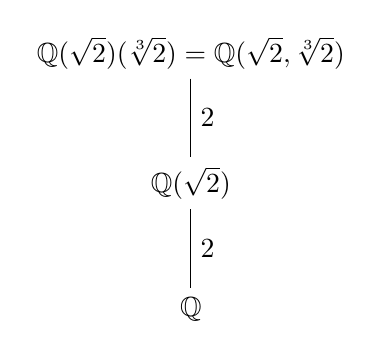
\begin{tikzpicture}
    \node (1) {$\mathbb{Q}(\sqrt{2})(\sqrt[3]{2}) = \mathbb{Q}(\sqrt{2}, \sqrt[3]{2})$};
    \node (2) [below = of 1] {$\mathbb{Q}(\sqrt{2})$};
    \node (3) [below = of 2] {$\mathbb{Q}$};

    \path 
    (1) edge node[right] {2} (2)
    (2) edge node[right] {2} (3);
  \end{tikzpicture}
\end{figure}
thus we have that $[\mathbb{Q}(\sqrt{2}, \sqrt[3]{2}) : \mathbb{Q}(\sqrt{2})] = 3$, and hence $[\mathbb{Q}(\sqrt{2}, \sqrt[3]{2}) : \mathbb{Q}] = 6$. The minimal polynomial of $\sqrt{2} + \sqrt[3]{2}$ has degree dividing 6.

\subparagraph{Example}

The fields of the form $K(\sqrt{a})$ and $K(\sqrt{a}, \sqrt{b})$ for non-square elements $a, b \in K$ are called quadratic\index{quadratic (extension)} and biquadratic\index{biquadratic (extension}) extensions of K.
\begin{figure}[H]
  \centering
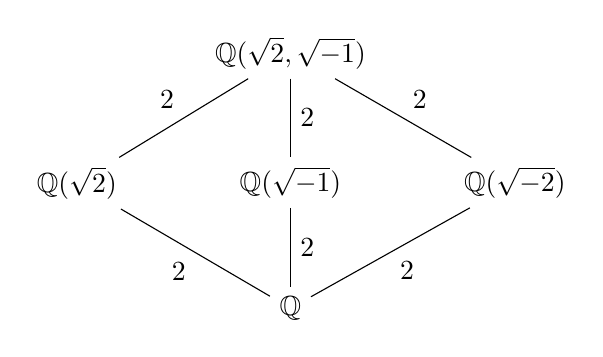
\begin{tikzpicture}
  \node (1) {$\mathbb{Q}(\sqrt{2}, \sqrt{-1})$};
  \node (2) [below left = of 1] {$\mathbb{Q}(\sqrt{2})$};
  \node (3) [below = of 1] {$\mathbb{Q}(\sqrt{-1})$};
  \node (4) [below right = of 1] {$\mathbb{Q}(\sqrt{-2})$};
  \node (5) [below = of 3] {$\mathbb{Q}$};

  \path
  (1) edge node[above left] {2} (2)
  (1) edge node[auto] {2} (3)  
  (1) edge node[auto] {2} (4)
  (2) edge node[below left] {2} (5)
  (3) edge node[auto] {2} (5)
  (4) edge node[auto] {2} (5);
\end{tikzpicture}
\end{figure}
hence $\mathbb{Q}(\sqrt{2}, \sqrt{-1})$ is a finite extension of degree 4, with basis for example $\{1, \sqrt{2}, \sqrt{-1}, \sqrt{-2}\}$.

\subparagraph{Remark}
Finite extensions are algebraic, but there exists infinite algebraic extensions.

\section{K-homomorphisms}

\begin{lemma}\label{lemma:11}
  If L is a field and $\tau : L \rightarrow L'$ be any ring homomorphism (where $L'$ is not a zero ring), then $\tau$ is injective.
\end{lemma}

\begin{proof}
  As $\ker \tau$ is an ideal of L not containing $1 \in L$ (as $\tau(1) = 1$), we have that $\ker \tau = \{0\}$.
\end{proof}

\begin{definition}\label{def:12}
  Let $L/K$, $L'/K$ be two etensions of K. A K-homomorphism\index{K-homomorphism} is a ring homomorphism from L to L' such that $\restr{\tau}{K} = \text{id}$. 

  The set of all K-homomorphisms is denoted by $\text{Hom}_k\left(L, L'\right)$.
\end{definition}

\subparagraph{Note}

All K-homomorphisms are injective. They are sometimes called embedding, and they are K-linear.

We are mainly interested in the set $\homset{L}{\mathbb{C}}$ when $K \subseteq L \subset \mathbb{C}$.

\subparagraph{Example}

\begin{description}
\item[$\mathbb{C}/\mathbb{R}$:] The $\mathbb{R}$-homomorphisms $\tau : \mathbb{C} \rightarrow \mathbb{C}$ are either:
  \begin{equation*}
    z \mapsto z \quad \text{or} \quad z \mapsto \overline{z}
  \end{equation*}
\item [$\mathbb{Q}(\sqrt{2})/\mathbb{Q}$:] The $\mathbb{Q}$-homomorphisms of $\mathbb{Q}(\sqrt{2} \rightarrow \mathbb{C}$. There are two, which verify:
  \begin{IEEEeqnarray*}{rCl}
    \tau_1 &:& \sqrt{2} \mapsto \sqrt{2} \\
    \tau_2 &:& \sqrt{2} \mapsto \sqrt{-2}
  \end{IEEEeqnarray*}
Note that since it is a ring homomorphism, it must send a root of P to a root of $P \in K[X]$.
\item[$\mathbb{Q}(\protect{\sqrt[3]{2}})/\mathbb{Q}$:] Let $\zeta^3=1$, $\zeta \neq 1$, then we have three $\mathbb{Q}$-homomorphisms:
  \begin{IEEEeqnarray*}{rCl}
    \tau_1 &:& \sqrt[3]{2} \mapsto \sqrt[3]{2} \\
    \tau_2 &:& \sqrt[3]{2} \mapsto \zeta\sqrt[3]{2} \\
    \tau_3 &:& \sqrt[3]{2} \mapsto \zeta^2\sqrt[3]{2}
  \end{IEEEeqnarray*}
in this case, the images $\text{Im} \tau_i$ are different subfields of $\mathbb{C}$.
\end{description}

\begin{definition}\label{def:13}
  \begin{enumerate}
  \item For a non-zero $P \in K[X]$ and an extension $L/K$, we denote by $\text{Root}_P(L)$ the set of all roots of P in L.
  \item Let $\alpha \in L$ be algebraic over K. A root of its minimal polynomial $P_\alpha$ over K in L, i.e. an element of $\text{Root}_{P_\alpha}(L)$, is called a conjugate\index{conjugate} of $\alpha$ in L over K.
  \end{enumerate}
\end{definition}

\begin{proposition}[Roots and Homomorphisms I]\label{prop:14}
  Let $F/K$, $E/K$ be two extensions of K and $\alpha \in F$ be algebraic over K. Then, we have a bijection:
  \begin{equation*}
    \homset[K]{K(\alpha)}{E} \rightarrow \rootset[P_\alpha]{E}
  \end{equation*}

In particular, we have that:
\begin{equation*}
  \cardinality{\homset[K]{K_\alpha}{E}} \leq [K(\alpha) : K]
\end{equation*}
\end{proposition}

\begin{proof}
  \begin{enumerate}
  \item We have a well-defined map:
    As $P_\alpha(\alpha) = 0$, and $\tau$ is a ring homomorphism such that $\restr{\tau}{K} = \text{id}$, we have that:
    \begin{equation*}
      P_\alpha(\tau(\alpha)) = \tau{}P_\alpha(\alpha) = 0
    \end{equation*}
(every K-homomorphism sends $\alpha$ to one of its conjugates in K)

\item It is injective:
All elements in $K(\alpha)$ are polynomials in $\alpha$ with coefficients in K, and $\restr{\tau}{K} = \text{id}$, the map is determined by $\tau(\alpha) \in E$.

\item It is surjective:
let $\beta \in \rootset[P_\alpha]{E}$, we define $\tau : K(\alpha) \rightarrow E$ satisfying $\tau(\alpha) = \beta$. Every $x \in K$ is written $x = P(\alpha)$ with $P \in K[X]$ and P is unique up to adding multiples of of $P_\alpha$ (i.e. any other choice of P is of the form $P + P_{\alpha}Q$), and $P_\alpha(\beta) = 0$ hence $P(\beta) \in E$ is well-defined. Hence let $\tau(x) = P(\beta)$, i.e.
\begin{IEEEeqnarray*}{rCl}
  \tau : K(\alpha) & \rightarrow & E \\
         P(\alpha) & \mapsto & P(\beta)
\end{IEEEeqnarray*}
this is a ring homomorphism, and $\restr{\tau}{K} = \text{id}$.

\item $\cardinality{\homset[K]{K(\alpha)}{E}} = \cardinality{\rootset[P_\alpha]{E}} \leq \deg P_\alpha = [K(\alpha) : K]$.
  \end{enumerate}
\end{proof}


%%% Local Variables: 
%%% mode: latex
%%% TeX-master: "Galois"
%%% End: 
\begin{example}[Uniform distribution]
Let $X_1, \dotsc, X_n$ be \iid $\Uniform[0, \theta]$. Let $T = \max X_i$.
$T$ is sufficient for $\theta$. Let $\tilde{\theta} = 2X_1$ be an unbiased estimator for $\theta$.
We have that:
\begin{IEEEeqnarray*}{rCl}
  \EE_\theta[\tilde{\theta} \given T = t] &=& 2\EE_\theta [X_1 \given \max X_i = t] \\
&=& 2 \left\{ \EE_\theta[X_1 \given \max X_i = t, \, X_1 = \max X_i]\PP(X_1 = \max X_i) + \EE_\theta[X_i \given \max X_i = t, \, X_1 \neq \max X_i]\PP(X_1 \neq \max X_i) \right\} \\
&=& 2 \left\{ t \frac{1}{n} + \frac{t}{2}\frac{n-1}{n} \right\} \\
&=& \frac{n+1}{n}t \mpunct{.}
\end{IEEEeqnarray*}
hence $\tilde{\theta} = \frac{n+1}{n} \max X_i$.
\end{example}

\section{Confidence intervals}
\emph{In this section, $\theta$ is scalar.}

\begin{definition}
  A $100\gamma\%$ confidence interval\index{confidence interval} (C.I.) for $\theta$ is a random interval $\left(A(\vec{X}), B(\vec{X})\right)$ such that:
\[
\PP_\theta \left( (\left(A(\vec{X}), B(\vec{X}) \ni \theta \right) \right) = \gamma
\]
no matter what the true value of $\theta$ may be.
\end{definition}

Note that it is the endpoints of the interval that are random.
Interpreting in terms of repeat sampling, if we calculate $\left(A(\vec{x}), B(\vec{x})\right)$ for a large number of samples $\vec{x}$, then approximately $100\gamma\%$ of them will cover the true $\theta$.

\begin{example}[label=ex:confidence_interval]
Let $X_1, \dotsc, X_n$ be \iid $\Normal(\theta, 1)$. Find a $95\%$ confidence interval for $\theta$.

We know $\overline{X} \sim \Normal(\theta, 1/n)$, so we have $\sqrt{n}(\overline{X} - \theta) \sim \Normal(0, 1)$, for all $\theta$. For any $z_1$, $z_2$, such that $\Phi(z_2) - \Phi(z_1) = 0.95$ (where $\Phi$ is the distribution function of $\Normal(0, 1)$), we have:
\[
\PP_\theta \left[ z_1 \leq \sqrt{n}\left(\overline{X} - \theta\right) < z_2 \right] = 0.95 \mpunct{,}
\]
i.e.
\[
\PP_\theta \left[ \overline{X} - \frac{z_2}{\sqrt{n}} < \theta < \overline{X} - \frac{z_1}{\sqrt{n}} \right] = 0.95 \mpunct{.}
\]
so we have that the following is a $95\%$ confidence interval for $\theta$:
\[
\left( \overline{X} - \frac{z_2}{\sqrt{n}}, \, \overline{X} - \frac{z_1}{\sqrt{n}} \right) \mpunct{.}
\]
We know that $\Normal(0, 1)$ is symmetric, so the shortest such interval obtained by using $z_2 = z_{0.025} = -z_1$ where $z_\alpha$ is the upper $100\alpha\%$ of $\Normal(0, 1)$.
\begin{figure}[h]
  \centering

  \begin{tikzpicture}[domain=-3:3,xscale=1.5,yscale=3]
    \draw[help lines, ->] (-3,0)--(3,0);
    \draw[help lines, ->] (0, -1)--(0, 1);

    \draw plot[id=nupp, samples=1000] function{exp(-x**2)/sqrt(2*pi)};

  \end{tikzpicture}

  \caption{$0.025$ Upper percentage point of $\Normal(0, 1)$}
  \label{fig:5.1}
\end{figure}
We find that $z_{0.025} = 1.96$, so the confidence interval is:
\[
\left(\overline{X} - \frac{1.96}{\sqrt{n}}, \overline{X} + \frac{1.96}{\sqrt{n}} \right) \mpunct{.}
\]
\end{example}

\vref{ex:confidence_interval} illustrates a procedure for finding confidence intervals:
\begin{enumerate}
\item Find a quantity $R(\vec{X}, \theta)$ such that the $\PP_\theta$-distribution of $R(\vec{X}, \theta)$ does not depend on $\theta$.
In the previous example, we had that $R(\vec{X}, \theta) = \sqrt{n}(\overline{X} - \theta)$. This is called the pivot\index{pivot}.

\item Write down a probability statement of the form:
\[
\PP_\theta(z_1 < R(\vec{X}, \theta) < z_2) = \gamma \mpunct{.}
\]
Usually, $z_1$, $z_2$ are percentage points.

\item Rearrange the inequalities inside the $\PP_\theta[ \, ]$ to find a confidence interval.
\end{enumerate}

\begin{example}[Normal variables]
Let $X_1, \dotsc, X_n$ be \iid $\Normal(0, \sigma^2)$. Find a $99\%$ confidence interval for $\sigma^2$.
From the probability review, we have that:
\[
\frac{1}{\sigma^2}\sum_{i=1}^n X_i^2 \sim \chi^2_n
\]
Recall $\chi^2_n(\alpha)$ denotes the upper $100\alpha\%$ point of $\chi^2_n$.
So we have that:
\[
\PP_{\sigma^2} \left[ \chi^2_n(0.995) < \frac{1}{\sigma^2}\sum_{i=1}^n X_i^2 < \chi^2_n(0.005) \right] = 0.99 \mpunct{,}
\]
i.e.
\[
\PP_{\sigma^2} \left[ \frac{\sum X_i^2}{\chi^2_n(0.005)} < \sigma^2 < \frac{\sum X_i^2}{\chi^2_n(0.995)} \right] \mpunct{.}
\]
Hence we have that the following is a $99\%$ confidence interval for $\sigma^2$:
\[
\left(\frac{\sum X_i^2}{\chi^2_n(0.005)}, \, \frac{\sum X_i^2}{\chi^2_n(0.995)} \right) \mpunct{.}
\]
If $n = 50$, we get $\chi^2_{50}(0.005) = 79.49$ and $\chi^2_{50} = 27.99$.
\end{example}

\begin{example}[Bernoulli variables]
Let $X_1, \dotsc, X_n$ be \iid $\Bernouilli(p)$ random variables. We know that the \mle of $p$ is $\hat{p} = \overline{X}$.
By the central limit theorem, we have that as $n$ tends to infinity,
\[
\frac{\sqrt{n}(\hat{p})}{\sqrt{p(1^-p)}} \rightarrow \Normal(0, 1) \mpunct{.}
\]
Hence we have that, for $n$ large:
\[
\PP_p \left[ \hat{p} - z_{\frac{1-\gamma}{2}}\sqrt{\frac{p(1-p)}{n}} < p < \hat{p} + z_{\frac{1-\gamma}{2}} \sqrt{\frac{p(1-p)}{n}} \right] \approxeq \gamma \mpunct{.}
\]
But $p$ is unknown, so we approximate $p$ by $\hat{p}$ to give an approximate asymptotic confidence interval for $p$:
\[
\left( \hat{p} - z_{\frac{1-\gamma}{2}}\sqrt{\frac{\hat{p}(1-\hat{p})}{n}}, \, \hat{p} + z_{\frac{1-\gamma}{2}}\sqrt{\frac{\hat{p}(1-\hat{p})}{n}} \right) \mpunct{.}
\]
\end{example}

Note that it is possible to have confidence regions for vector parameters (see example sheet 1). Also, if $\left(A(\vec{X}), B(\vec{X})\right)$ is a $100\gamma\%$ confidence interval for $\theta$ and $\tau(\theta)$ is a monotone increasing function of $\theta$, then $\left(\tau(A(\vec{X})), \tau(B(\vec{X}))\right)$ is a $100\gamma\%$ confidence interval for $\tau(\theta)$.



%%% Local Variables:
%%% mode: latex
%%% TeX-master: "statistics"
%%% End:

\begin{theorem}[Separability]\label{thm:18}
  Let $F/K$ be a finite extensions inside $\mathbb{C}$. Then, we have:
  \begin{equation*}
    \cardinality{\homset{F}{\mathbb{C}}} = [F : K]
  \end{equation*}
\end{theorem}

\begin{proof}
  Let $F = K(\alpha_1, \ldots, \alpha_n)$ (by prop \eqref{prop:10}). If $n = 1$, then this reduces to prop \eqref{prop:15}. Proceed by induction $n$: let $L = K(\alpha_1, \ldots, \alpha_{n-1})$, $F = L(\alpha)$ with $\alpha = \alpha_n$, and consider the restriction map:
  \begin{IEEEeqnarray*}{rCl}
    \homset{F}{\mathbb{C}} &\rightarrow& \homset{L}{\mathbb{C}} \\
    \rho & \mapsto \restr{\rho}{L}
  \end{IEEEeqnarray*}
By proposition \eqref{prop:17}, the inverse image of each $\tau \in \homset{L}{\mathbb{C}}$ has cardinality $\cardinality{\rootset[\tau{}P_\alpha]{\mathbb{C}}}$. Now $\tau{}P_\alpha$ is irreducible in $\tau(L)[X]$ (where $P_\alpha$ is the minimal polynomial of $\alpha$ over L), as it is the image of $P_\alpha \in L[X]$ under the ring isomorphism $L[X] \rightarrow \tau(L)[X]$ extending $\tau : L \rightarrow \tau(L)$. Hence, we have that:
\begin{equation*}
   \cardinality{\rootset[\tau{}P_\alpha]{\mathbb{C}}} = \deg \tau{}P_\alpha = \deg P_\alpha  \qquad \text{(by prop \eqref{prop:15})}
\end{equation*}
but we also have that:
\begin{equation*}
 \deg P_\alpha = [L(\alpha) : L] \qquad \text{(by prop \eqref{prop:7})}
\end{equation*}
thus, we have:
  \begin{IEEEeqnarray*}{rClr}
   \cardinality{\homset{F}{\mathbb{C}}} &=& [L(\alpha) : L] \cdot \cardinality{\homset{L}{\mathbb{C}}}& \\
    &=& [F : L][L : K] & \text{by induction hypothesis} \\
    &=& [F : K] & \text{by tower law} 
  \end{IEEEeqnarray*}
 \end{proof}

We have also proved the following:

\begin{lemma}\label{lemma:19}
  Let $F/K$ be a finite extension inside $\mathbb{C}$ and $K \subseteq L \subseteq F$. Then, the map:
  \begin{IEEEeqnarray*}{rCl}
    \homset{F}{\mathbb{C}} & \rightarrow & \homset{L}{\mathbb{C}} \\
    \rho & \mapsto & \restr{\rho}{L}
  \end{IEEEeqnarray*}
is surjective, i.e. one can extend every K-homomorphism $\tau : L \rightarrow \mathbb{C}$ to F.
\end{lemma}

\begin{theorem}[Primitive element\index{primitive element (theorem)} theorem]\label{thm:20}
  Every finite extensions inside $\mathbb{C}$ is simple.
\end{theorem}

\begin{proof}
  We prove the simplicity of every finite $F/K$ with $\cardinality{K}$ infinite and satisfying the following (in our case, by theorem \eqref{thm:18}):

if $K \subseteq L \subseteq F$, there exists an extension $E/K$ such that $\cardinality{\homset{L}{E}} = [L : K]$.

Let $F = K(\alpha_1, \ldots, \alpha_n)$ (prop. \eqref{prop:10}. We show that $K(\alpha_1, \ldots, \alpha_i)/K$ simple by induction on $i$. By induction hypothesis, suffices to prove that $L = K(\alpha, \beta) \subseteq F$ is simple over K.

For $\gamma \in L$ with $K\subseteq K(\gamma) \subseteq L$, we have:
\begin{equation*}
  \card{\homset{K(\alpha)}{E}} \leq [K(\alpha) : K] \leq [L : K] = \card{\homset{L}{E}}
\end{equation*}
and equality implies $L = K(\alpha)$.

Hence let $d = [L : K]$ and $\homset{L}{E} = \{ \tau_1, \ldots, \tau_d \}$, it suffices to find $\gamma \in L$ such that $\restr{\tau_i}{K(\alpha)}$ are distinct elements of $\homset{K(\alpha)}{E}$, i.e. $\tau_1(\alpha), \ldots, \tau_d(\alpha)$ all distinct.

We try $\gamma$ of the form $\gamma = \alpha{}x + \beta$, with $x \in K$. We need that:
\begin{IEEEeqnarray*}{rCl}
  0 &\neq& \prod_{i \neq j} \left(\tau_i(\gamma) - \tau_j{\gamma}\right) \\
  &=& \prod_{i \neq j}\left[ \left(\tau_i(\alpha)x + \tau_i(\beta)\right) - \left(\tau_j(\alpha)x + \tau_j(\beta)\right)\right] \\
  &=& \prod_{i \neq j}\left(\left(\tau_i(\alpha)-\tau_j(\alpha)\right)x + \left(\tau_i(\beta) - \tau_j(\beta)\right)\right)
\end{IEEEeqnarray*}
So it will do as long as x is not a root of:
\begin{equation*}
  \prod_{i \neq j}\Big(\big(\tau_i(\alpha)-\tau_j(\alpha)\big)X + \big(\tau_i(\beta) - \tau_j(\beta)\big)\Big) \in E[X]
\end{equation*}
which is not identically zero as $\tau_i(\alpha) \neq \tau_j(\alpha)$ or $\tau_i(\beta) \neq \tau_j(\beta)$ for $i \neq j$ (as $\tau_i \neq \tau_j$, and $L = K(\alpha, \beta)$), hence has only finitely many roots. As $\card{K}$ is infinite, we win.
\end{proof}

\subparagraph{Example}

\begin{enumerate}
\item $\mathbb{Q}(\sqrt{2}, \sqrt{3}) = \mathbb{Q}(\sqrt{2} + \sqrt{3})$
\item $\mathbb{Q}(\sqrt{2}, \sqrt[3]{2}) = \mathbb{Q}(\sqrt{2} + \sqrt[3]{2})$
\end{enumerate}

\section{Galois extensions}

\begin{definition}\label{def:21}
  Let $L/K$, $L'/K$ be extensions. If a K-homomorphism $\tau : L \rightarrow L'$ is a bijection (of sets) then $\tau^{-1} : L' \rightarrow L$ is also a K-homomorphism, and we say that $\tau$ is a K-isomorphism\index{K-ismorphism}. A K-isomorphism $L \rightarrow L$ is called a K-automrphism\index{K-automorphism}, and theset of all K-automorphisms of $L$ is a denoted by $\autset{L}$, a subset of $\homset{L}{L}$. It is a group under composition.
\end{definition}

\begin{lemma}
  \label{lemma:22}
  \begin{enumerate}
  \item If there is a K-homomorphism $\tau : L \rightarrow L'$, then $[L : K] \leq [L' : K]$.
  \item If $[L : K] = [L' : K] < \infty$, then every $\tau \in \homset{L}{L'}$ is a K-isomorphism. In particular, $\homset{L}{L} = \autset{L}$ for finite $L/K$.
  \item If $L/K$ is a finite extension inside $\mathbb{C}$, then $\card{\autset{L}} \leq [L : K]$
  \end{enumerate}
\end{lemma}

\begin{proof}
  Recall that K-homomorphisms are injective (lemma \eqref{lemma:11}). 

  Let $V$, $V'$ be vector spaces over K. If there exists K-linear injective maps $V \rightarrow V'$ then $\dim_K \leq \dim_K V'$. An injective K-linear map $V \rightarrow V'$ is bijective if $\dim_K V = \dim_K V' < \infty$ by rank-nullity. This proves the first two claims.

Now, consider:
\begin{equation*}
  \autset{L} = \homset{L}{L} \subseteq \homset{L}{\mathbb{C}}
\end{equation*}
but we have that $\card{\homset{L}{\mathbb{C}}} = [L : K]$.
\end{proof}

\begin{definition}
  \label{def:23}
  A finite extension $L/K$ is called Galois\index{Galois} if:
  \begin{equation*}
    \card{\autset{L}} = [L : K]
  \end{equation*}
\end{definition}
In this case $\autset{K}$ is called the Galois group\index{Galois group} and denoted by $\Gal{L/K}$.

\begin{proposition}
  \label{prop:24}
  Let $L/K$ be a finite extension inside $\mathbb{C}$. The following are equivalent:

  \begin{enumerate}
  \item $L/K$ is Galois \label{prop:24:i}
  \item Every K-homomorphism $\tau : L \rightarrow \mathbb{C}$ maps $L$ into itself. \label{prop:24:ii}
  \item $\forall \alpha \in L$, every conjugate of $\alpha$ over K is in L.\label{prop:24:iii}
  \item $L = K(\alpha_1, \ldots, \alpha_n)/K$, and every conjugate of $\alpha_i (1 \leq i \leq n)$ over K is in L. \label{prop:24:iv}
  \end{enumerate}
\end{proposition}

\begin{proof}
  \begin{description}
  \item[\ref{prop:24:i} $\Leftrightarrow$ \ref{prop:24:iii}] By the proof of lemma \eqref{lemma:22}, we have that:
    \begin{equation*}
      L/K \ \text{Galois} \Leftrightarrow \homset{L}{L} = \homset{L}{\mathbb{C}}
    \end{equation*}
  \end{description}
  
\end{proof}
%%% Local Variables: 
%%% mode: latex
%%% TeX-master: "Galois"
%%% End: 

\begin{theorem}[Local maximum principle]
If $f : B_a(r) \rightarrow \CC$ holomorphic, for some ball $B_a(r)$, and $\abs{f(z)} \leq \abs{f(a)}$ for all $z \in B_a(r)$, then $f$ is constant.
I.e. ``a holomorphic $f$ cannot achieve an interior local maximum''.
\end{theorem}

\begin{proof}
Fix some $0 < \rho < r$. We can write
\begin{IEEEeqnarray*}{rCl}
\abs{f(a)} &=& \abs*{ \int_0^1 f\left(a + \rho e^{2 \pi i t}\right) dt} \\
&\leq& \sup_{\abs{z - a} = \rho} \abs*{f(z)}  \leq \abs*{f(z)} \mpunct{.}
\end{IEEEeqnarray*}
Hence we deduce that $\abs{f(z)} = \abs{f(a)}$ for all $z \in \{ z : \abs{z - a} = \rho \}$.
Thus, we have that $\abs{f(z)}$ constant on $B_a(r)$, hence we can deduce that $f$ is constant.

\end{proof}

\begin{theorem}[name=Liouville's theorem, label=thm:liouville]
  Let $f : \CC \rightarrow \CC$ be holomorphic (i.e. $f$ entire).
If $f$ is bounded, then $f$ is constant.
\end{theorem}

Note that this is obviously false in $\RR$, for example $\cos x$, $\sin x$.

\begin{proof}
  Suppose $\abs{f(z)} \leq M$ for all $z \in \CC$.
Let $z_1, z_2 \in \CC$, and let $R \geq 2 \max \{ \abs{z_1}, \abs{z_2} \}$.
We have the following:
\begin{IEEEeqnarray*}{rCl}
\abs*{f(z_1) - f(z_2)} &=& \abs*{\frac{1}{2 \pi i} \int_{\partial B_0(R)} \left(\frac{f(w)}{w - z_1} - \frac{f(w)}{w - z_2}\right) dw} \\
&=& \abs*{\frac{1}{2 \pi i} \int_{\partial B_0(R)} \frac{f(w)(z_1 - z_2)}{(w - z_1)(w-z_2)} dw } \\
&\leq& \frac{1}{2 \pi} 2 \pi R \frac{M \abs{z_1 - z_2}}{(R/2)^2} \\
&=& \frac{4M}{R}\abs{z_1 - z_2} \mpunct{.}
\end{IEEEeqnarray*}
As this holds for all $R$ large enough, $f(z_1) = f(z_2)$.
\end{proof}

\begin{theorem}[name=Fundamental theorem of algebra, label=thm:fta]
Every non-constant polynomial has at least one root in $\CC$ (i.e. a non-constant polynomial $p(z)$ factorizes into linear factors over $\CC$).
\end{theorem}

\begin{proof}
  Let $P(z) = a_nz^n + a_{n-1}z^{n-1} + \dotsb + a_0$ with $a_n \neq 0$ (and $n > 0$).
As $\abs{z} \rightarrow \infty$ we have that $\abs{P(z)} \rightarrow \infty$ sine the leading term dominates.
Hence, there exists $R > 0$ such that for all $\abs{z} > R$,, we have $\abs{P(z)} > 1$.

Suppose for contradiction that $P(z)$ has no root.
Let $f(z) = 1/P(z)$. This is holomorphic on $\CC$ as $P(z) \neq 0$ for $z \in \CC$.
As $f$ is continuous, we have that $f$ is bounded on the closed bounded set $\overline{B_0(R)}$.
However, on $\CC \setminus \overline{B_0(R)}$, we have $\abs{P(z)} \geq 1$ hence $\abs{f(z)} \leq 1$.
Thus, we have that $f$ is bounded on $\CC$, and hence is constant by \cref{thm:liouville}, from which we deduce that $P(z)$ is constant, which is contradictory.
\end{proof}

\paragraph{Remark}

There is no algebraic proof of \cref{thm:fta}.
The construction of $\ZZ$ from $\NN$, and the one of $\QQ$ from $\ZZ$ are algebraic, and the construction of $\CC$ from $\RR$ is algebraic.
However, the construction of $\RR$ from $\QQ$ is essentially an \emph{analytic} process, and other choices of metric would yield different completions.

\section{Cauchy's formula for derivatives}

\begin{theorem}[Cauchy's formula for derivatives]
Let $U$ e a domain, and $f$ holomorphic on $U$.
Suppose $\overline{B_a(r)} \subseteq U$, then for every $n \geq 0$, $f^{(n)}(a)$ exists, and
\[
f^{(n)}(a) = \frac{1}{2 \pi i} \int_{\partial B_a(r)} \frac{f(w)}{(w-a)^{n+1}} dw \mpunct{.}
\]
In particular, $f$ is infinitely differentiable on $U$.
\end{theorem}

Note that if $n = 0$, this is \cref{thm:cauchy_integral}.

\paragraph{Remarks}

We have that $f$ is holomorphic at $z \in U$ if and only $\Re f$ and $\Im f$ satisfy the Cauchy-Riemann equations and $\Re f$, $Im f$ differentiable.

\paragraph{Cauchy's proof of Cauchy's theorem}

Let $f$ be holomorphic on a domain $U$. Write $f(z) = u(x, y) = i v(x, y)$ and assume $u$, $v$ have continuous partial derivatives.
Then, for $\gamma$ a closed contours, we have that $\int_\gamma f(z) dz = 0$.

\begin{proof}
We have the following equalities
\begin{IEEEeqnarray*}{rCl}
\int_\gamma f(z) \: dz &=& \int_\gamma (u + iv)(dx + idy) \\
&=& \int_\gamma u dx - v dy + i \int_\gamma v dx + u dy \\
&=& \int_D -\left(\frac{\partial u}{\partial y} + \frac{\partial v}{\partial x}\right) \: dx \: dy + i \int_D \left( \frac{\partial u}{\partial x} - \frac{\partial v}{\partial y} \right) \: dx \: dy \quad \text{(by Green's theorem)} \mpunct{.}
\end{IEEEeqnarray*}
\end{proof}

%%% Local Variables:
%%% mode: latex
%%% TeX-master: "complex_analysis"
%%% End:

\section{Taylor's theorem}

\begin{theorem}[name=Taylor's theorem, label=thm:taylor]
  Let $f : B_a(r) \rightarrow \CC$ be holomorphic. Then $f$ has a convergent power series representation on $B_a(r)$
\[
f(w) = \sum_{n=0}^\infty c_n(w - a)^n \mpunct{.}
\]
The coefficients are given by
\[
c_n = \frac{f^{(n)}(a)}{n!} = \frac{1}{2 \pi i} \int_{\partial B_a(\rho)} \frac{f(z)}{(z-a)^{n+1}} \: dz
\]
where $0 < \rho < r$.
\end{theorem}

\begin{remark}
We saw directly that a convergent power series was infinitely differentiable, and that the coefficients of power series are given by $c_n = f^{(n)}(a)/n!$.
\end{remark}

\begin{proof}
Consider a point $w$ with $\abs{w - a} < \rho < r$. By \cref{thm:cauchy}, we have that:
\[
f(w) = \frac{1}{2 \pi i}\int_{\partial B_a(\rho)} \frac{f(z)}{z - w} dz \mpunct{.}
\]
Now remark that we have
\[
\frac{1}{z - w} = \frac{1}{(z - a)\left( 1 - \frac{w - a}{z - a} \right)} = \sum_{n = 0}^\infty \frac{(w-a)^n}{(z-a)^{n+1}} \mpunct{.}
\]
By comparison to a geometric progression, this converges uniformly on $\abs{z - a} = \rho$.
As we have that the Riemann integral behaves nicely with respect to uniform convergence, we can exchange summation of a uniformly convergent power series and its integration.
Hence, we have that
\begin{IEEEeqnarray*}{rCl}
f(w) &=& \frac{1}{2 \pi i} \int_{\partial B_a(\rho)} f(z) \sum_{n=0}^\infty \frac{(w-a)^n}{(z- a)^{n+1}} dz \\
&=& \sum_{n=0}^\infty \left( \frac{1}{2 \pi i} \int_{\partial B_a(\rho)} \frac{f(z)}{(z-a)^{n+1}} \right) (w-a)^n \mpunct{.}
\end{IEEEeqnarray*}
which exhibits a convergent power series representing $f$.
\end{proof}

Contrast that result with the fact that  $exp \left(-\frac{1}{x^2}\right)$ has identically zero ``Taylor series'' at $0$. This gives a proof of Cauchy's formula for derivatives, but it is a bit sleight-of-hand. We sketch an alternative.

\begin{proof}
  We want to prove that:
\[
f^{(n)}(a) = \frac{n!}{2 \pi i} \int_\gamma \frac{f(z)}{(z-a)^{n+1}} dz \mpunct{.}
\]
  Proof by induction on $n$. Suppose that the result holds for $n = k$.
  We have that
  \begin{IEEEeqnarray*}{rCl}
f^{(k)}(a + h) - f^{(k)}(a) &=& \frac{k!}{2 \pi i} \int_{\partial B_a(2r)} f(w) \left( \frac{1}{(w - a -h)^{k+1}} - \frac{1}{(w-a)^{k+1}} \right) dw \\
&=& \frac{k!}{2 \pi i} \int_{\partial B_a(2r)} f(w) \left( (k+1) \int_{ [a, a+h] } (w - \xi)^{-(k+2)} d\xi \right) dw \mpunct{.}
  \end{IEEEeqnarray*}

Now consider
\[
F(h) = \frac{f^{(k)}(a+h) - f^{(k)}(a)}{h} - \frac{(k+1)!}{2 \pi i}\int_{\partial B_a(2r)} \frac{f(w)}{(w-a)^{k+2}} dw \mpunct{.}
\]
and use the fundamental theorem of calculus a second time to obtain
\[
F(h) = \frac{(k+2)!}{2 \pi i h} \int_{\partial B_a(2r)} f(w) \left( \int_{[a, a+h]} \int_{[a, \xi]} (w - \tau)^{-(k+3)} d\tau \: d\xi \right) \: dw \mpunct{.}
\]
Now we know that $f$ is holomorphic, hence continuous and bounded on $\overline{B_a(2r)}$, say $\abs{f(z)} < M$. We have that $\xi \in [a, a+h]$ implies $\abs{w - \tau} \leq r$ for $w \in \partial B_a(2r)$, and that $\tau \in [a, a+h]$ implies that
\[
\abs{F(h)} \leq \frac{(k+2)!}{2 \pi \abs{h}} 4 \pi r M \frac{abs{h}^2}{r^{h+3}} = O(\abs{h}) \mpunct{.}
\]
\end{proof}

\begin{corollary}[Morera's theorem]
Let $U$ be a domain and $f : U \rightarrow \CC$ continuous. If we have that
\[
\int_\gamma f(z) dz = 0
\]
for all closed paths $\gamma$, then $f$ is holomorphic on $U$.
\end{corollary}

Note that this is a ``converse'' to Cauchy's theorem but we do not assume $U$ is simply connected.

\begin{proof}
As $\int_\gamma f(z) dz = 0$ for all closed paths $\gamma$, we know that $f$ has an antiderivative $F(z)$, defined as
\[
F(z) = \int_{a_0}^z f(w) dw \mpunct{.}
\]
with $F'(t) = f(t)$.
By definition, $F(z)$ is holomorphic, as it is clearly differentiable with derivative $f$.
So $F(z)$ is infinitely differentiable, and in particular, $f(z) = F'(z)$ is holomorphic.
\end{proof}

Let $f : B_a(r) \rightarrow \CC$ be holomorphic. We have $f(z) = \sum_{n \geq 0} c_n(z-a)^n$.
Observe that if $\forall n, c_n  = 0$ then $f \equiv 0$ on $B_a(r)$.
Otherwise, there exists a smallest $N > 0$ such that $c_N \neq 0$.
Then $f(z) = (z - a)^N g(z)$ where $g(z) = \sum_{n \geq N}c_n(z-a)^{n-N}$ and $g(a) \neq 0$.

\begin{definition}
  If $N > 0$, we say hat $f$ has a zero of order $N$ at $a$. We have that
\[
N = min \{ n \mid f^{(n)}(a) \neq 0 \}
\]
\end{definition}

\begin{proposition}[name=Principle of isolated zeros]
  If $f : B_a(r) \rightarrow \CC$ is holomorphic and $f$ is not identically $0$, then there exists some $0 \rho < r$ such that $f(z) \neq 0$ for $z \in B_a(\rho) \setminus \{ a \}$.
\end{proposition}

\begin{proof}
  If $f(a) \neq 0$, this is true by continuity of $f$.
  If there exists a zero of order $N$, then the result holds by continuity of $g$, where $f(z) = (z-a)^N g(z)$.
\end{proof}

%%% Local Variables:
%%% mode: latex
%%% TeX-master: "complex_analysis"
%%% End:

\paragraph{Example 2.3}
Single normal sample, testing a given mean, known variance: Z-test.

Let $X_1, \dotsc, X_n$ be \iid $\Normal(\mu, \sigma_0^2)$, with $\sigma_0^2$ known.
Let $H_0 : \mu = \mu_0$ and $H_1 : \mu \neq \mu_0$ with $\mu_0$ known.
Then, we have that $\Theta_0  = \{ \mu_0 \}$, hence we have that
\[
\sup_{\mu \in \Theta_0} L(\mu; \vec{x}) = L(\mu_0, \vec{x}) = f(\vec{x}; \mu_0) \mpunct{.}
\]
On the other hand, we have that
\[
\sup_{\mu \in \Theta} L(\mu; \vec{x}) = \sup_{\mu \in \RR} L(\mu; \vec{x}) = L(\hat{\mu}; \vec{x}) = f(\vec{x}; \hat{\mu}) \mpunct{,}
\]
where $\hat{\mu}$ is the maximum likelihood estimator, i.e. $\hat{\mu} = \overline{x}$.
Hence, we have that
\[
\Lambda_{\vec{x}} (H_0; H_1) = \frac{\left( \frac{1}{\sqrt{2 \pi \sigma_0^2}} \right)^n \exp \left\{ -\frac{1}{2 \sigma_0^2} \sum (x_i - \hat{\mu})^2 \right\}}{\left( \frac{1}{\sqrt{2 \pi \sigma_0^2}} \right)^n \exp \left\{ -\frac{1}{2 \sigma_0^2} \sum (x_i - \mu_0)^2 \right\}} \mpunct{,}
\]
so we deduce that
\begin{IEEEeqnarray*}{rCl}
2 \log \Lambda_{\vec{x}} (H_0, H_1) &=& \frac{1}{\sigma_0^2} \left[ \sum (x_i - \mu_0)^2 - \sum (x_i - \overline{x})^2 \right] \\
&=& \frac{n \big(\overline{x} - \mu_0\big)^2}{\sigma_0^2} \mpunct{.}
\end{IEEEeqnarray*}

We reject $H_0$ if $\Lambda$ and hence $2 \log \Lambda$ is large, i.e. if $\Lambda \big(\overline{x} - \mu_0\big)^2/\sigma_0^2$ is large, or equivalently if
\[
\frac{\sqrt{n}}{\sigma_0} \abs*{\overline{x} - \mu_0}
\]
is large.
Under $H_0$, we have that $\frac{sqrt{n}}{\sigma_0}\Big(\overline{X} - \mu_0\Big) \sim \Normal(0, 1)$.
Hence we reject $H_0$ if $\abs*{\sqrt{n}\big(\overline{x} - \mu_0\big)/\sigma_0} > Z_{\alpha/2}$ for a size $\alpha$ test.
This is a two-tailed test\index{two-tailed test}.

Note that since $n\Big(\overline{X} - \mu_0\Big)^2/\sigma_0^2 \sim \xi^2_1$ under $H_0$, so the above test is equivalent to rejecting $H_0$ if $n \big(\overline{x} - \mu_0 \big)^2/\sigma_0^2 > \xi^2_1(\alpha)$ (check that $z_{\alpha/2} = \xi^2_1(\alpha)$).

\subparagraph{Wiks' theorem}
It turns out that we can still use generalised likelihood ratio tests even when we cannot find the exact null distribution of the test statistic.
Suppose $\dim \Theta = k$ and that $\Theta_0$ imposes $p$ independent restrictions so that $\dim \Theta_0 = k - p$.
We write $\abs{\Theta} = k$ and $\abs{\Theta_0} = k - p$.
We say $\Theta$ has ``$k$ free parameters'' and $\Theta_0$ has ``$k-p$ free parameters''.

Under regularity conditions, with $\vec{X} = \big(X_1, \dotsc, X_n\big)$ with $X_i$ \iid, we have that if $H_0$ is true, then $2 \log \Lambda_{\vec{x}} (H_0; H_1)$ is approximately distributed as $\xi^2_p$ for large $n$, and if $H_0$ is not true, then $2 \log \Lambda$ tends to be larger (Wiks' theorem).

In example 2.3, we have that $\abs{\Theta} = 1$, and $\abs{\Theta_0} = 0$, so we have that $p = \abs{\Theta} - \abs{\Theta_0}$, and we have seen that $2 \log \Lambda \sim \xi^2_1$.

\section{Goodness-of-fit test}

Suppose we wish to test whether our data comes from a particular parametric family $\{ f_X(\cdot, \theta) \quad \theta \in \Theta \}$.
Partition $\curlyX$ into sets $A_1, \dotsc, A_k$ and let $p_i = \PP (X_i \in A_i)$ and $p_i(\theta) = \int_{A_i} f_X(x, \theta) \: dx$.

Consider testing $H_0 : p_i  = p_i(\theta) \text{ for } i = 1, \dotsc, k \text{ for some } \theta$ versus $H_1 : p_i \geq 0, \sum p_i = 1$.
This is a goodness-of-fit test\index{goodness-of-fit test} and we carry it out using a generalised likelihood ratio test.

Let $N_i = \text{number of observations in } A_i$. Under $H_1$, we have that $(N_1, \dotsc, N_k) \sim \text{Multinomial}(n, p_1, \dotsc, p_k)$, and the likelihood is such that
\[
L(p_1, \dotsc, p_k) \propto p_1^{n_1} \dotsm p_k^{n_k}
\]
and the log-likelihood is
\[
\ell (p_1, \dotsc, p_k) = \text{constant} + \sum_{i=1}^k n_i \log p_i \mpunct{.}
\]
We maximise the log-likelihood subject to $\sum p_i = 1$ by considering the Lagrangian
\[
\mathscr{L} = \sum_{i=1}^k n_i \log p_i - \lambda(\sum p_i - 1) \mpunct{.}
\]
We find the maximum likelihood estimators $\hat{p_i} = n_i/n$.

Under $H_0$, we can find $\hat{\theta}$ (the \mle of $\theta$) by maximising $\sum n_i \log p_i(\theta)$ with respect to $\theta$. Then, we have that
\begin{IEEEeqnarray*}{rCl}
2 \log \Lambda_{\vec{x}} (H_0; H_1) &=& 2 \log \left( \frac{\hat{p_1}^{n_1} \dotsm \hat{p}^n_k}{p_1(\hat{\theta})^{n_1} \dotsm p_k(\hat{\theta})^{n_k}} \right) \\
&=& 2 \sum n_i \log \left( \frac{\hat{p_i}}{p_i(\hat{\theta})} \right) \\
&=& 2 \sum n_i \log \left( \frac{n_i}{n p_i(\theta)} \right) \mpunct{,}
\end{IEEEeqnarray*}
the generalised likelihood ratio test rejects $H_0$ if $2 \log \Lambda > \xi^2_{k - 1 - \abs{\Theta_0}}$.

If we let $o_i = n_i$ (the observed number in $A_i$), $e_i = n p_i(\hat{\theta})$ (the ``expected'' number in $A_i$ under $H_0$) and $\delta_i = o_i - e_i$ so that $o_i = e_i + \delta_i$.
If $H_0$ is true, we expect $\delta_i << e_i$.
Then, we have that
\begin{IEEEeqnarray*}{rCl}
  2 \log \Lambda_{\vec{x}} (H_0; H_1) &=& 2\sum_{i=1}^k o_i \log \left( \frac{o_i}{e_i} \right) \\
&=& 2 \sum (e_i + \delta_i) \log \left( 1 + \frac{\delta_i}{e_i} \right) \\
&=& 2 \sum \left( \delta_i + \frac{\delta_i^2}{e_i} - \frac{\delta_i^2}{2e_i} + o(\delta_i^2) \right) \\
&\approx& \sum \frac{\delta_i^2}{e_i} \\
&=& \sum \frac{(o_i - e_i)^2}{e_i} \mpunct{.}
\end{IEEEeqnarray*}

%%% Local Variables:
%%% mode: latex
%%% TeX-master: "statistics"
%%% End:

We call $T = \sum \frac{(o_i - e_i)^2}{e_i}$ the Pearson's chi-squared statistic\index{Pearson's chi-squared statistic} and we reject $H_0$ if $T > \chi^2_{k-1-\abs{\Theta}}(\alpha)$.

\begin{example}[name=Mendel's peas, label=ex:2.4]
We consider an experiment whereby we cross $556$ smooth yellow peas with wrinked green female peas. From the progeny, we let
\begin{itemize}
\item $N_1$ be the number of smooth yellow peas,
\item $N_2$ be the number of smooth green peas,
\item $N_3$ be the number of wrinkled yellow peas,
\item $N_4$ be the number of wrinkled green peas.
\end{itemize}
We test the goodness of fit test of the model:
\[
H_0 : (p_1, p_2, p_3, p_4) = (9/16, 3/16, 3/16, 1/16) \mpunct{.}
\]
Observe that $(n_1, n_2, n_3, n_4) = (315, 108, 102, 31)$. \\
We find that $(e_1, e_2, e_3, e_4) = (312.75, 104.25, 104.25, 34.75)$, hence we have that
\[
2 \log \Lambda = 0.618 \text{ and } \sum \frac{(o_i - e_i)^2}{e_i} = 0.604 \mpunct{.}
\]

Now, we have that $\abs{\Theta_0} = 0$ and $\abs{\Theta_1} = 4 - 1 = 3$, hence we must refer our test statistic to $\chi^2_3$.
We have that $\chi^2_3 (0.05) = 7.815$, so neither value is significant at the $5\%$ level, and there is no evidence against Mendel's theory.
In fact, the $p$-value is approximately $\PP(\chi^2_3 > 0.6) \approx 0.9$, the values are ``very ordinary''.
\end{example}

\section{Testing independence in contingency tables\label{sec:2.6}}
Contingency tables\index{contingency table} arise when observations or individuals are classified according to two or more criteria.

\begin{example}[label=ex:2.5]
$500$ people with recent car changes were asked about their previous and new cars.
The results of the poll are presented in \vref{table:ex:2.5}.
This is a two-way contingency table: each person is classified according to previous car size and new car size.

\begin{table}[h]
  \centering
  \begin{tabular}{rrrr}
    \toprule
    & \multicolumn{3}{c}{New car} \\
    \cmidrule{2-4}
    Previous car & Large & Medium & Small \\
    \midrule
    Large & $56$ & $52$ & $42$ \\
    Medium & $50$ & $83$ & $67$ \\
    Small & $18$ & $51$ & $81$ \\
    \bottomrule
  \end{tabular}
  \caption{Number of people per old and new car size.}
  \label{table:ex:2.5}
\end{table}
\end{example}

Consider a two-way contingency table with $r$ rows and $c$ columns.
Let $p_{ij}$ be the probability that a randomly selected individual is classified in row $i$ and column $j$, i.e. is in the $(i, j)$ cell of the table.
Let
\begin{IEEEeqnarray*}{rCl}
p_{i+} ( = p_{i\cdot} ) &=& \sum_{j=1}^c p_{ij} = \PP(\text{in row $i$}) \mpunct{,} \\
p_{+j} ( = p_{\cdot j} ) &=& \sum_{i = 1}^r p_{ij} = \PP(\text{in column $j$}) \mpunct{.}
\end{IEEEeqnarray*}
We must have that $p_{++} = \sum_{i, j} p_{ij} = 1$, i.e. $\sum_i p_{i+} = 1 = \sum_j p_{+j}$.

Suppose a random sample of $n$ individuals is taken.
Let $N_{ij}$ be the number of these in the $(i, j)$ cell.
Let $N_{i+} = \sum_j N_{ij}$, $N_{+j} = \sum_i N_{ij}$, $N_{++} = \sum_{i, j} N_{ij}$.
Then, we have that
\[
(N_{11}, N_{12}, \dotsc, N_{1c}, N_{21}, \dotsc, N_{2c}, \dotsc, N_{rc}) \sim \Multinomial (n; p_{11}, p_{12}, \dotsc, p_{1c}, p_{21}, \dotsc, p_{2c}, \dotsc, p_{rc}) \mpunct{.}
\]

We test $H_0 : \text{the two classifications are independent}$, i.e.
\[
H_0 : p_{ij} = p_{i+}p_{+j} \text{ for } i = 1, \dotsc, r \quad j = 1, \dotsc, c
\]
with constraints $\sum_i p_{i+} = 1$ and $\sum_j p_{+j} = 1$,
versus $H_1 : p_{ij} \text{ unrestricted}$ (except for the usual normalization conditions).

Under $H_1$, the maximum likelihood estimators are $\hat{p_{ij}} = n_{ij}/n$ (as obtained in \ref{sec:2.5}).

Under $H_0$, we have that $L \propto \prod (p_{i+}p_{+j})^{n_{ij}}$. Use Lagrangian methods with:
\[
\mathscr{L} = \sum_i n_{i+} \log p_{i+} + \sum_j n_{+j} \log p_{+j} - \lambda\left(\sum p_i - 1\right) - \mu\left(\sum p_{+j} - 1\right) \mpunct{.}
\]
We the find that $\hat{p}_{i+} = n_{i+}/n$ and $\hat{p}_{+j} = n_{+j}/n$.

Let $o_{ij} = n_{ij}$, $e_{ij} = n\hat{p}_{i+}\hat{p}_{+j} = n_{i+}n_{+j}/n$.
Now we have that
\begin{IEEEeqnarray*}{rCl}
2 \log \Lambda &=& 2 \sum_{i = 1}^r \sum_{j=1}^c o_{ij} \log \left(\frac{o_{ij}}{e_{ij}}\right) \\
&\approx& T = \sum_{i = 1}^r \sum_{j=1}^c \frac{(o_{ij} - e_{ij})^2}{e_{ij}} \mpunct{.}
\end{IEEEeqnarray*}
We have that $\abs{\Theta} = rc - 1$, and $\abs{\Theta_0} = (r-1) + (c-1)$, and hence
\[
\abs{\Theta} - \abs{\Theta_0} = rc - 1 - (r - 1) - (c - 1) = (r-1)(c-1) \mpunct{.}
\]
Thus $2 \log \Lambda$ and $T$ are compared to $\chi^2_{(r-c)(c-1)} (\alpha)$.

\begin{example}[continues=ex:2.5]
Now suppose that we wish to test $H_0$, the hypothesis that the new and previous car sizes are independent.

\begin{table}[h]
  \centering
  \begin{tabular}{rrrr}
    \toprule
    & \multicolumn{3}{c}{New car} \\
    \cmidrule{2-4}
    Previous car & Large & Medium & Small \\
    \midrule
    Large & 37.2 & 55.8 & 57.0 \\
    Medium & 49.6 & 74.4 & 76.0 \\
    Small & 37.2 & 55.8 & 57.0 \\
    \bottomrule
  \end{tabular}
  \caption{Expected values for car ownership under $H_0$}
  \label{tab:ex:2.5.2}
\end{table}

We obtain, using the previous formula (and the values of $e_{ij}$ as in \vref{tab:ex:2.5.2})
\[
\sum_{i, j} \frac{(o_{ij}-e_{ij})^2}{e_{ij}} = 36.20 \mpunct{.}
\]
We have $(3-1)(3-1)=4$ degrees of freedom, hence we find that $\chi^2_4 (0.05) = 9.488$ and $\chi^2_4 (0.01) = 13.28$.
The observed value of $36.20$ is significant at the $1\%$ level, hence we have strong evidence against $H_0$.
We can thus conclude that the new and present car sizes are not independent.

\begin{table}[h]
  \centering
  \begin{tabular}{rSSS}
    \toprule
    & \multicolumn{3}{c}{New car} \\
    \cmidrule{2-4}
    Previous car & {Large} & {Medium} & {Small} \\
    \midrule
    Large & 3.08 & -0.51 & -1.99 \\
    Medium & 0.06 & 1.00 & -1.03 \\
    Small & -3.14 & -0.64 & 3.18 \\
    \bottomrule
  \end{tabular}
  \caption{Deviation from expected value for car ownership}
  \label{tab:ex:2.5.3}
\end{table}

In fact, we can consider the values of $(o_{ij} - e_{ij})/e_{ij}$ in each cell (as in \vref{tab:ex:2.5.3}), and we see that:
\begin{itemize}
\item more owners of large cars than expected under $H_0$ bought another large car,
\item more owners of small cars than expected under $H_0$ bought another small car,
\item fewer than expected under $H_0$ changed from a small to a large car.
\end{itemize}
\end{example}

\section{Testing homogeneity in contingency tables}
\label{sec:2.7}

\begin{example}
\begin{table}[h]
  \centering
  \begin{tabular}{rrrr}
    \toprule
    & Improved & No difference & Worse \\
    \midrule
    Placebo & 18 & 17 & 15 \\
    Half dose & 20 & 10 & 20 \\
    Full dose & 25 & 13 & 12 \\
    \bottomrule
  \end{tabular}
  \caption{Results of the experiment}
  \label{tab:ex:2.6}
\end{table}

$150$ patients are randomly divided into three groups of $50$ patients. The experiment is carried out, and the result are reported in \vref{tab:ex:2.6}.
Let $H_0$ be the hypothesis that ``the probability of `improved' is the same for each of the three treatment groups, and so are the probabilities of `no difference' and `worse' ''.
$H_0$ is the hypothesis that we have homogeneity between the rows.

\emph{the carrying out of the test is left as an exercise to the reader.}
\end{example}

In general, we have independent observations from $r$ multinomial distributions, each with $c$ categories.
\[
(N_{i1}, \dotsc, N_{ic}) \sim \Multinomial(n_{i+}, p_{i1}, \dotsc, p_{ic}) \mpunct{.}
\]
We test the following hypothesis
\[
H_0 : p_{1j} = p_{2j} = \dotsc = p_{rj} ( = p_j \text{, say}), \ j = 1, \dotsc, c
\]
with the constraint that $\sum_j p_j = 1$, against the hypothesis:
\[
H_1 : p_{ij} \text{ unrestricted}
\]
with the constraint $p_{i+} = 1$ for $i = 1, \dotsc, r$.

Using a generalized likelihood ratio test, we find that
\[
2 \log \Lambda = 2 \sum_{i = 1}^r \sum_{j = 1}^c n_{ij} \log \left( \frac{n n_{ij}}{n_{i+}n_{+j}} \right) \mpunct{,}
\]
which is identical to the $2 \log \Lambda$ as in \cref{sec:2.6}, and similarly for $T$.
Here, we have that $\abs{\Theta_0} = c-1$, $\abs{\Theta} = r(c-1)$, so that $\abs{\Theta} - \abs{\Theta_0} = (r-1)(c-1)$.
Hence, both $2 \log \Lambda$ and $T$ are referred to $\chi^2_{(r-1)(c-1)} (\alpha)$.

%%% Local Variables:
%%% mode: latex
%%% TeX-master: "statistics"
%%% End:

\section{Confidence sets and hypothesis tests}
Confidence intervals/sets can be obtained by ``inverting'' hypothesis tests, and vice versa.

\begin{definition}
The acceptance region\index{acceptance region} $A$ of a test is the complement of the critical region, i.e. $A = \overline{C}$.
\end{definition}

\begin{theorem}
We have the following ``conversion'' from confidence intervals/sets to hypothesis tests:
\begin{enumerate}
\item   Suppose that for every $\theta_0 \in \Theta$ there is a size $\alpha$ test of $H_0 : \theta = \theta_0$.
Denote the acceptance region by $A(\theta_0)$.
Then the set $I(\vec{X}) = \{ \theta \mid \vec{X} \in A(\theta) \}$ is a $100(1 - \alpha)\%$ confidence set for $\theta$.
\item Conversely suppose $I(\vec{X})$ is a $100(1-\alpha)\%$ confidence set for $\theta$.
Then $A(\theta_0) = \{ \vec{X} \mid \theta_0 \in I(\vec{X}) \}$ is the acceptance region for a size $\alpha$ test of $H_0 : \theta = \theta_0$.
\end{enumerate}
\end{theorem}

\begin{proof}
  Note first that $\theta_0 \in I(\vec{X})$ if and only if $\vec{X} \in A(\theta_0)$ in both cases.
\begin{enumerate}
\item Since the test is size $\alpha$, we have for all $\theta_0 \in \Theta$
\[
\PP_{\theta_0} ( I (\vec{X}) \ni \theta_0 ) = \PP_{\theta_0} (\vec{X} \in A(\theta_0)) = 1 - \alpha \mpunct{.}
\]
\item Since $I(\vec{X})$ is a $100(1-\alpha)\%$ confidence region for $\theta$, we have, for all $\theta_0 \in \Theta$
\[
\PP_{\theta_0}( \vec{X} \in A(\theta_0) ) = \PP_{\theta_0} ( I(\vec{X}) \ni \theta_0 ) = 1 - \alpha \mpunct{.}
\]
$A(\theta_0)$ defines a test of size $\alpha$.
\end{enumerate}
\end{proof}

\chapter{Linear Models}

\section{The multivariate normal distribution}
A random vector\index{random vector} $\vec{X} = (X_1, \dotsc, X_n)$ has mean $\vec{\mu} = \EE (\vec{X}) = (\EE(X_1), \dotsc, \EE(X_n)) = (\mu_1, \dotsc, \mu_n)$, and a covariance matrix\index{covariance matrix} $\cov \vec{X} = \EE \left[ (\vec{X} - \vec{\mu})(\vec{X} - \vec{\mu})^T \right]$ with the $(i, j)$ element being $\cov (X_i, X_j)$ (provided the relevant expectations exist).

For a $m \times n$ matrix $A$, we have:
\begin{equation}
  \label{eq:3.1}
\EE [A\vec{X}] = A \vec{\mu} \text{ and } \cov (A\vec{X}) = A (\cov \vec{X}) A^T \mpunct{.}
\end{equation}

Define $\cov( \vec{V}, \vec{W} )$ to be the matrix with the $(i, j)$ element being $\cov (V_i, W_j)$. Then we have that
\[
\cov (A\vec{X}, B\vec{X}) = A (\cov \vec{X}) B^T \mpunct{.}
\]

$\vec{X}$ has a multivariate normal distribution\index{multivariate normal} if, for every $\vec{t} \in \RR^n$, the random variable $\vec{t}^t\vec{X}$ has a normal distribution.
If $\EE(\vec{X}) = \vec{\mu}$ and $\cov \vec{X} = \Sigma$, we write $\vec{X} \sim \Normal_n (\vec{\mu}, \Sigma)$.
Note that $\Sigma$ is symmetric (as $\cov (X_i, X_j) = \cov(X_j, X_i)$), and it is positive semi-definite (as we have that by \eqref{eq:3.1}, $\vec{t}^t\Sigma\vec{t} = \var \vec{t}^t \vec{X} \geq 0$).
By \eqref{eq:3.1}, we know that $\vec{t}^t\vec{X} \sim \Normal(\vec{t}^t\vec{\mu}, \vec{t}^t\Sigma\vec{t})$, hence we know that $\vec{t}^t\vec{X}$ has moment generating function
\[
M_{\vec{t}^t\vec{X}}(s) = \EE\left[ e^{s \vec{t}^t\vec{X}} \right] = \exp \left\{ \vec{t}^t\vec{\mu}s + \frac{1}{2} \vec{t}^t\Sigma\vec{t} s^2 \right\}\mpunct{.}
\]
Hence $\vec{X}$ has m.g.f.
\begin{equation}
  \label{eq:3.2}
M_{\vec{X}}(\vec{t}) \stackrel{\text{def}}{=} \EE \left[e^{\vec{t}^T\vec{X}}\right] = M_{\vec{t}^t\vec{X}}(1) = \exp \left\{ \vec{t}^T\vec{\mu} + \frac{1}{2}\vec{t}^T\Sigma\vec{t} \right\} \mpunct{.}
\end{equation}

\begin{proposition}
The multivariate normal\index{multivariate normal} distribution has the following properties
\begin{enumerate}
\item If $\vec{X} \sim \Normal_n(\vec{\mu}, \Sigma)$ and $A$ is a $m \times n$ matrix, then we have
\[
A\vec{X} \sim \Normal_m(A\vec{\mu}, A \Sigma A^T) \mpunct{.}
\]
\item If $\vec{X} \sim \Normal(\vec{0}, \sigma^2 I)$ where $I$ denotes the identity matrix, then we have
\[
\frac{\norm{X}^2}{\sigma^2} = \frac{\vec{X}^T\vec{X}}{\sigma^2} = \frac{\sum X_i^2}{\sigma^2} \sim \chi^2_n \mpunct{.}
\]
\end{enumerate}
\end{proposition}

\begin{proof}
The first proof is left as an exercise to the reader.
The second part is immediate from the definition of $\chi^2_n$.
\end{proof}

\begin{proposition}
  Let $\vec{X} \sim \Normal_n(\vec{\mu}, \Sigma)$, and let $\vec{X} = (\vec{X_1}, \vec{X_2})$, where $\vec{X_1}$ is $n_1 \times 1$ and $X_2$ is $n_2 \times 1$ where $n = n_1 + n_2$.
Similarly partition $\vec{\mu} = (\vec{\mu_1}, \vec{\mu_2})$ and partition $\Sigma$ as:
\[
\Sigma =
\begin{pmatrix}
  \Sigma_{11} & \Sigma_{12} \\ \Sigma_{21} & \Sigma_{21}
\end{pmatrix} \mpunct{.}
\]
Then we have the following:
\begin{enumerate}
\item $\vec{X_1} \sim \Normal_{n_1}(\vec{\mu_1}, \Sigma_{11})$,
\item $X_1$ and $X_2$ are independent if and only if $\Sigma_{12} = 0$.
\end{enumerate}
\end{proposition}

\begin{proof}
  The first part is left as an exercise to the reader.

From \eqref{eq:3.2}, we have that
\[
M_{\vec{X}} (\vec{t}) = \exp \left\{ \vec{t}^T\vec{\mu} + \frac{1}{2} \vec{t}^T\Sigma\vec{t} \right\} \mpunct{.}
\]
Write $\vec{t} = (\vec{t_1}, \vec{t_2})$ where $\vec{t_1}$ is $n_1 \times 1$ and $\vec{t_2}$ is $n_2 \times 1$. Then we have that:
\[
M_{\vec{X}} (\vec{t}) = \exp \left\{ \vec{t_1}^T\vec{\mu_1} + \vec{t_2}^T\vec{\mu_2} + \frac{1}{2} \vec{t_1}^T\Sigma_{11}\vec{t_1} + \frac{1}{2} \vec{t_2}^T\Sigma_{22}\vec{t_2} + \frac{1}{2} \vec{t_1}^T\Sigma_{12}\vec{t_2} + \frac{1}{2} \vec{t_2}^T\Sigma_{21}\vec{t_1} \right\} \mpunct{.}
\]

From the first part, we know that $M_{X_i}(t_i) = \exp \left\{ \vec{t_i}^T\vec{\mu_i} + \frac{1}{2}\vec{t_i}^T\Sigma_{ii} \vec{t_i} \right\}$.
So $M_{\vec{X}}(\vec{t}) = M_{\vec{X_1}}(\vec{t_1})M_{\vec{X_2}}(\vec{t_2})$ for all $\vec{t}$ if and only if $\Sigma_{12}$.
\end{proof}

When $\Sigma$ is positive definite, $\vec{X}$ has a probability density function
\[
f_{\vec{X}}(\vec{x}; \vec{\mu}, \Sigma) = \frac{1}{\abs{\Sigma}^{1/2}} \left(\frac{1}{\sqrt{2 \pi}} \right)^n \exp \left\{ -\frac{1}{2} (\vec{x} - \vec{\mu})^T\Sigma^{-1}(\vec{x} - \vec{\mu}) \right\} \mpunct{.}
\]

\section{Normal random samples}
We know consider the following quantities for normal data:
\begin{IEEEeqnarray*}{rCl}
  \overline{X} &=& \frac{1}{n}\sum_{i=1}^n X_i \\
  S_{xx} &=& \sum_{n=1}^n (X_i - \overline{X})^2 = \sum_{i=1}^n X_i^2 - n\overline{X}^2
\end{IEEEeqnarray*}


%%% Local Variables:
%%% mode: latex
%%% TeX-master: "statistics"
%%% End:

\begin{theorem}[label=thm:3.3]
 If $X_1, \dotsc, X_n$ are \iid $\Normal(\mu, \sigma^2)$ then
 \begin{enumerate}
 \item $\overline{X} \sim \Normal(\mu, \sigma^2/n)$
 \item $S_{xx} \sim \sigma^2 \chi^2_{n-1}$,
 \item $\overline{X}$ and $S_{xx}$ are independent.
 \end{enumerate}
\end{theorem}

\begin{proof}
  We know $\vec{X} \sim \Normal_n (\vec{\mu}, \sigma^2 I)$ where $\vec{\mu} = \mu\vec{1}$, where $\vec{1}$ is the $n \times 1$ vector of ones.
Let $A$ be such that:
\[
A =\begin{pmatrix}
  \frac{1}{\sqrt{n}} & \frac{1}{\sqrt{n}} & \frac{1}{\sqrt{n}} & \frac{1}{\sqrt{n}} & \dots & \frac{1}{\sqrt{n}} \\

  \frac{1}{\sqrt{2 \times 1}} & - \frac{1}{\sqrt{2 \times 1}} & 0 & 0 & \dots & 0 \\
  \frac{1}{\sqrt{3 \times 1}} & \frac{1}{\sqrt{3 \times 2}} & - \frac{2}{\sqrt{3 \times 2}} & 0 & \dots & 0 \\
  \vdots & \vdots & \vdots & \vdots & \ddots & \vdots \\
  \frac{1}{\sqrt{n(n-1)}} & \frac{1}{\sqrt{n(n-1)}} & \frac{1}{\sqrt{n(n-1)}} & \frac{1}{\sqrt{n(n-1)}} & \dots & \frac{-(n-1)}{\sqrt{n(n-1)}}
\end{pmatrix}
\]
$A$ is orthogonal, as the rows form an orthogonal basis of $\RR^n$.
Let $\vec{Y} = A \vec{X}$.
By \cref{prop:3.1}, we have that
\[
\vec{Y} \sim \Normal_n (A \vec{\mu}, A \sigma^2 I A^T) \sim \Normal_n(A \vec{\mu}, \sigma^2 I) \mpunct{.}
\]
We also have $A\vec{\mu} = (\sqrt{n}\mu, 0, 0, \dotsc, 0)$, so we have $Y_1 \sim \Normal(\sqrt{n}\mu, \sigma^2)$ and $Y_i \sim \Normal(0, \sigma^2)$, for $i \geq 2$ by \cref{prop:3.2}, and $Y_1, \dotsc, Y_i$ are independent.

Note that we have
\[
Y_1 = (A\vec{X})_1 = \frac{1}{\sqrt{n}} \sum_{i = 1}^n = \sqrt{n} \overline{X} \mpunct{.}
\]
hence we have $\sqrt{n}\overline{X} \sim \Normal(\sqrt{n}\mu, \sigma^2)$, hence we deduce that $\overline{X} = \Normal(\mu, \sigma^2/n)$.

Note further that we have
\begin{IEEEeqnarray*}{rCl}
  Y_2^2 + \dotsb + Y_n^2 &=& \vec{Y}^T\vec{Y} - Y_1^2 \\
&=& \vec{X}^T A^TA\vec{X} - n \overline{X}^2 \\
&=& \sum_{i = 1}^n X_i^2 - n\overline{X}^2 \\
&=& S_{xx} \mpunct{.}
\end{IEEEeqnarray*}
hence we have $S_{xx} = Y_2^2 + \dotsb + Y_n^2 = \sigma^2\chi_{n-1}^2$ by definition of $\chi^2$.

Now we have that $Y_1$ and $(Y_2, \dotsc, Y_n)$ are independent by \cref{prop:3.2}, so $\overline{X}$ and $S_{xx}$ are independent.
\end{proof}

\begin{definition}
  Suppose $Z \sim \Normal(0, 1)$ and $Y \sim \chi^2_k$, where $Z$ and $Y$ are independent. Then the quantity
\[
T = \frac{Z}{\sqrt{Y/k}}
\]
has a $t$-distribution\index{t-distribution} on $k$ degrees of freedom.
We write $T \sim t_k$.
\end{definition}

\begin{example}
  Suppose $X_1, \dotsc, X_n$ are \iid $\Normal(\mu, \sigma^2)$, where $\mu$ and $\sigma^2$ are unknown.
From \cref{thm:3.3}, we know that $\sqrt{n}(\overline{X} - \mu)/\sigma \sim \Normal(0, 1)$, and that $S_{xx} / \sigma^2 \sim \chi^2_{n-1}$, with both quantities independent.
Hence, we have that the quotient
\begin{IEEEeqnarray*}{rCl}
T &=& \frac{\sqrt{n}(\overline{X} - \mu)/\sigma}{\sqrt{S_{xx}/(\sigma^2(n-1))}} \\
&=& \frac{\sqrt{n}(\overline{X} - \mu)}{\sqrt{\frac{S_{xx}}{n-1}}} \sim t_{n-1} \mpunct{.}
\end{IEEEeqnarray*}
Let $\tilde{\sigma}^2 = S_{xx}/(n-1)$. Then a $100(1-\alpha)\%$ confidence intervals for $\mu$ is found from
\[
1- \alpha = \PP\left(-t_{n-1}(\alpha/2) \leq \frac{\sqrt{n}(\overline{X} - \mu)}{\tilde{\sigma}} \leq t_{n-1}(\alpha/2)\right)
\]
where $t_{n-1}(\alpha/2)$ is the upper $100\alpha/2\%$ point of the $t_{n-1}$ distribution, and has endpoints $\overline{X} = \pm \tilde{\sigma}t_{n-1}(\alpha/2)/\sqrt{n}$.
See the example sheet for the use of $T$ in hypothesis testing.
\end{example}

\begin{definition}
  Suppose that $V \sim \chi^2_r$ and $W \sim \chi^2_s$ are independent random variables.
Then the following quantity
\[
F = \frac{V/r}{W/s}
\]
has an $F$-distribution\index{F-distribution} on $r$ and $s$ degrees of freedom.
We write $F \sim F_{r, s}$.
\end{definition}

If $X \sim F_{r, s}$, then we have that $1/X \sim F_{s, r}$ from the definition.
If $T \sim t_n$, then $T^2 \sim F_{1, n}$.
See example sheet for the use of $F$ in statistical inference.

\section{The linear model}
\label{sec:3.3}

Linear models can be used to explain or model the relationship between a response\index{response} (or output\index{output} or dependent\index{dependent}) variable $Y$ and one or more explanatory variables\index{explanatory variable} (or covariates\index{covariate} or predictors\index{predictor}).

For example, we could model the way in which car insurances claim sizes depend on the age of the driver, the region in where the policy holder lives, etc.
Here, the claim size is the response, and the age and region are explanatory variables.

In the linear model\index{linear model}, we assume that $Y_1, \dotsc, Y_n$ are $n$ observations of the response variable. The model is
\begin{equation}
  \label{eq:3.3}
Y_i  = \beta_1 x_{i1} + \dotsb + \beta_p x_{ip} + \epsilon_i \quad i = 1, \dotsc, n
\end{equation}
where $\beta_1, \dotsc, \beta_p$ are unknown parameters ($n > p$), and $x_{i1}, \dotsc, x_{ip}$ are the values of $p$ covariates for the i\textsuperscript{th} (assumed known).
$\epsilon_1, \dotsc, \epsilon_n$ are independent (or uncorrelated) random variables with mean $0$ and variance $\sigma^2$.

%%% Local Variables:
%%% mode: latex
%%% TeX-master: "statistics"
%%% End:


\paragraph{Example}

Let us compute the following integral:
\[
\int_0^\infty \frac{1}{1 + x^4} \: dx
\]

Let $\gamma_R$ be the closed contour comprising $[-R, R] \subseteq \RR$ and the arc of semicircle of radius $R$. $f(z) = 1/(1 + z^4)$ has poles at $e^{i \pi / 4}$ and $e^{3 i \pi /4}$ inside $\gamma$.

Hence we have that
\[
\int_{\gamma_R} \frac{1}{1 + z^4} \: dz = 2 \pi i \sum_{p_i} \mathrm{Residues}
\]
but we have that
\[
\int_{\gamma_R} \frac{1}{1 + z^4} \: dz = \int_{-R}^R \frac{1}{1 + x^4} \: dx + \int_0^\pi \frac{i R e^{i\theta}}{1 + R^4 e^{4 i \theta}} \: d\theta \mpunct{.}
\]

The integral over the semicircle has order $O(1/R^3)$, and hence vanishes as $R \rightarrow \infty$. Now we have that
\[
\Res_f(p_i) = \frac{1}{4 p_i^3}
\]
and since $p_i^4 = -1$, we have $\Res_f (p_i) = -p_i/4$, so we have that
\[
\int_0^\infty \frac{1}{1 + x^4} \: dx = \frac{\pi}{2 \sqrt{2}} \mpunct{.}
\]

\paragraph{Example}
Compute the following integral
\[
\int_{-\infty}^\infty \frac{\cos x}{1 + x + x^2} \: dx \mpunct{.}
\]
We know that $1/(1 + z + z^2)$ has a simple pole at $e^{2 \pi i /3}$.
Note that $\cos z$ becomes large on a semicircle of radius $R$ (it takes value $O(e^R)$), thus we take instead
\[
f(z) = \frac{e^{i z}}{1 + z + z^2} \mpunct{.}
\]

Then, we have that, putting $\gamma_R$ the semicircle of radius $R$
\begin{IEEEeqnarray*}{rCl}
\int_{\gamma_R} f(z) dz &=& \int_{-R}^R f(x) dx + \int_0^\pi f(R e^{i\theta})i R e^{i\theta} d\theta \\
&=& 2 \pi i \Res_f (e^{2 \pi /3}) \\
&=& 2 \pi i \frac{e^{i w}}{2w + 1} \\
&=& \frac{2 \pi}{\sqrt{3}} (e^{i (-1 + \sqrt{3}i)/2}) \mpunct{.}
\end{IEEEeqnarray*}
where $w = e^{2 \pi i / 3}$.

Note that
\[
\Re \left(\int_{-R}^R f(x) dx \right) = \int_{-\infty}^\infty \frac{\cos x}{1 + x + x^2} dx \mpunct{.}
\]
We also have that
\[
\abs*{\int_0^\pi f(R e^{i\theta}) i R e^{i\theta} d\theta} \leq \int_0^\pi \frac{R e^{- R \sin \theta}}{\abs{1 + R e^{i \theta} + R^2 e^{2 i \theta}}} d\theta \mpunct{.}
\]

\paragraph{Example}
Compute the following integral
\[
\int_0^\infty \frac{\cos x}{x} dx \mpunct{.}
\]

Consider the contour $\gamma_{R}$, then we have that this contour runs through a pole of the integrand. Hence, we replace $\gamma_R$ by a modified contour $\gamma_{R, \epsilon}$.

\begin{lemma}
 Let $f$ be holomorphic on $B_a(r) \setminus \{ a \}$ with a simple pole at $a$.
 Let $0 < \epsilon < r$, and let $\gamma_\epsilon : [\alpha, \beta] \rightarrow \CC$ be $t \mapsto a + \epsilon e^{it}$.
 Then we have that
\[
\lim_{\epsilon \rightarrow 0} \int_{\gamma_\epsilon} f(z) dz = (\beta - \alpha)i \Res_f (a) \mpunct{.}
\]
\end{lemma}

\begin{proof}
  We write $f(z) = \frac{c}{z - a} + g(z)$ where $g$ is holomorphic, and $c = \Res_f (a)$.
  We have that
\[
\abs*{\int_{\gamma_\epsilon} g(z) dz} \leq (\beta - \alpha) \epsilon \sup_{\gamma_\epsilon} \abs{ g(z) } \mpunct{.}
\]
but $g$ is holomorphic, hence in particular continuous and bounded in a neighbourhood of $a$.
Thus, we have that this quantity tends to $0$ as $\epsilon$ tends to $0$.
Hence, we have that
\[
\lim_{\epsilon \rightarrow 0} \int_{\gamma_\epsilon} f(z) dz = \lim_{\epsilon \rightarrow 0} \int_{\gamma_\epsilon} \frac{c}{z - a} dz \mpunct{.}
\]
This is equal to
\[
c \lim_{\epsilon \rightarrow 0} \int_\alpha^\beta \frac{1}{\epsilon e^{i t}} \epsilon e^{i t} dt = i (\beta - \alpha) c \mpunct{.}
\]
\end{proof}

\begin{lemma}[Jordan's lemma]
 Let $f$ be holomorphic on $\{ \abs{z} > r \}$ and suppose that on this region, $z f(z)$ is bounded.
 Let $\gamma_R : [0, \pi] \rightarrow \CC$ be the path $t \mapsto R e^{i t}$.
 Then, for all $\alpha > 0$ we have that
\[
f(z) e^{i \alpha z} dz \rightarrow 0 \text{ as } R \rightarrow \infty \mpunct{.}
\]
\end{lemma}

\begin{proof}
  Suppose $\abs{f(z)} \leq C/\abs{z}$ for sufficiently large $\abs{z}$.
  On $(0, \pi/2]$, we have that
\[
\frac{d}{d\theta} \left(\frac{\sin \theta}{\theta}\right) = \frac{\theta \cos \theta - \sin \theta}{\theta^2} \leq 0 \mpunct{.}
\]
Hence $\sin \theta / \theta$ is decreasing, and $\sin t \geq 2 t/\pi$ for $t \in [0, \pi/2]$.
On $\gamma_R$ we have that $\abs{e^{i \alpha z}} = e^{- \alpha R \sin t}$, but we have that
\[
e^{- \alpha R \sin t} \leq
\begin{cases}
  e^{-2 \alpha R t / \pi} & 0 \leq t \leq \pi/2  \mpunct{,}\\
  e^{-2 2 R t' /\pi} & 0 \leq t' = \pi - t \leq \pi /2 \mpunct{.}
\end{cases}
\]
then we have that
\
\begin{IEEEeqnarray*}{rCl}
\abs*{ \int_0^{\pi/2} e^{i \alpha R e^{it}} f(R e^{it}) i R e^{it} dt } \\
&\leq& \int_0^{\pi/2} e^{- \alpha R t} C dt \\
&=& \frac{1}{\alpha R} (1 - e^{- \alpha R \pi /2}) \mpunct{.}
\end{IEEEeqnarray*}
\end{proof}
%%% Local Variables:
%%% mode: latex
%%% TeX-master: "complex_analysis"
%%% End:


\paragraph{Corrigendum}

Compute the following integral
\[
\int_0^\infty \frac{\sin x}{x} dx \mpunct{.}
\]
The function $\sin (z) /z$ has a removable singularity at $0$.
If $f(z) = \sin(z) / z$, then on $\gamma_R$ the integrand is of order $O(e^R/R)$, which does not tend to $0$ as $R \rightarrow \infty$.
Instead, we consider $f(z) = e^{iz}/z$. This function has a simple pole at $0$.
Hence take the contour that avoids the origin by an $\epsilon$ semi-circle, and use Jordan's lemma to see that the integral is bounded.
Putting everything together, we have that
\[
\int_0^\infty \frac{\sin x}{x} dx = \frac{\pi}{2} \mpunct{.}
\]

\section{More contour integrals}

\paragraph{Example}
Compute the following integral:
\[
\int_0^{\pi/2} \frac{1}{1 + \sin^2 t} dt
\]

Recall that $\sin t = (e^{it} - e^{-it}) / 2i = (z + 1/z) / 2i$, hence if $z = e^{it}$, we have $dt = \frac{dz}{iz}$.
Moreover, we have that
\[
\int_0^{\pi/2} \frac{1}{1 + \sin^2 t} dt = \frac{1}{4}\int_0^{2\pi} \frac{1}{1 + \sin^2 t} dt \mpunct{.}
\]
Hence we get
\[
\int_0^{\pi/2} \frac{1}{1 + \sin^2 t} dt = \frac{1}{4} \int_\gamma \frac{1}{1 + \frac{(z - 1/z)^2}{-4}} \frac{dz}{iz} = \frac{1}{4} \int_\gamma \frac{iz}{z^4 - 6 z^2 + 1} dz
\]
the quadratic $y^2 - 6y + 1$ has roots at $3 \pm 2 \sqrt{2}$, so the poles of $z / (z^4 - 6z^2 + 1)$ occur at $1 \pm \sqrt{2}$ and $-1 \pm \sqrt{2}$.
These are simple poles, and the residues are $-i\sqrt{2}/16$, and we have that
\[
\int_0^{\pi/2} \frac{1}{1 + \sin^2 t} dt = \frac{\pi}{\sqrt{2} \mpunct{.}
\]
Note that using the above substitution, we can compute ``any'' integral of the shape
\[
\int_0^{2\pi} \frac{P (\sin t)}{Q (\sin t)} dt
\]
where $P$ and $Q$ are polynomials.

\paragraph{Example}
Compute the following integral:
\[
\int_{-\infty}^{+\infty} \frac{e^{a x}}{\cosh x} dx
\]
with $-1 < a < 1$.
Note that we have
\[
\cosh z = 0 \Leftrightarrow e^z + e^{-z} = 0 \Leftrightarrow z = \left( n + \frac{1}{2}\right) i \pi \mpunct{.}
\]

As an alternative to summing residue contributions from many poles, note that $\cosh (x + i \pi) = - \cosh x$.
Now consider a large rectangle of height $i \pi$ running from $-S$ to $R$, sitting on the real axis. Let $\gamma_+$ be the vertical part of the contour, we have that
\[
\int_{\gamma_+} f(z) dz = \int_0^^\pi \frac{e^{a(R + iy)}}{\cosh(R + iy)} i dy}  \mpunct{.}
\]

We estimate the integral by
\begin{IEEEeqnarray*}{rCl}
  \abs*{\int_{\gamma_+} f(z) dz } &\leq& \int_0^{2\pi} \frac{ 2 e^{aR} }{ \abs*{ e^{R + iy} + e^{-R + iy}}} dy \\
&\leq \int_0^\pi \frac{2 e^{aR} }{\abs*{e^R - e^{-R}}} dy \mpunct{.}
\end{IEEEeqnarray*}
which tends to $0$ as $R \rightarrow \infty$, as we have that $a < 1$.
Similarly, we have that $\int_{\gamma_-} f(z) dz \rightarrow 0$ as $S \rightarrow \infty$ as $a > -1$.
As $R, S \rightarrow \infty$, we have that
\[
\int_{-\infty}^\infty \frac{e^'{ax}}{\cosh x} dx + \int_{+ \infty}^{- \infty} \frac{e^{a i \pi}e^{a x}}{\cosh (x + i\pi)} dx = 2 \pi i \Res_f ( i \pi / 2 ) \mpunct{.}
\]
We have that $f(z) = e^{az}/\cosh(z)$ has residue $e^{ap}/\sinh(p)$ at $p = i \pi /2$, hence we have the final result is:
\[
\int_{-\infty}^{+\infty} \frac{e^{ax}}{\cosh x} dx (1 + e^{a i \pi}) = 2 \pi i (- i e^{i a \pi /2}) \mpunct{,}
\]
i.e. we have
\[
\int_{-\infty}^{+\infty} \frac{e^{a x}}{\cosh x} dx = \pi \mathop{sec} \left(\frac{\pi a}{2} \right) \mpunct{.}
\]

\paragraph{Example}
Compute the following integral
\[
\int_0^\infty \frac{\log x}{1 + x^2} dx
\]
We can only define $\log z$ in a slit plane.
Hence we consider the contour that avoids the origin and runs $i \pi$ above the negative real axis.
We have that
\[
\int_\epsilon^R \frac{\log x}{1 + x^2} dx + \int_{\gamma_R} f(z) dz + \int_R^\epsilon \rac{\log (x) + i \pi}{1 + x^2} (-dx) + \int_{\gamma_\epsilon} f(z) dz = (2 \pi i) \pi/4 \mpunct{.}
\]

On the large semicircle, we have that
\[
\abs*{\int f(z) dz} \leq \int_0^\pi \abs*{ \frac{ \log R + i  \theta}{1 + R^2 + e^{2 i \theta}}} R d\theta = O(R^{-1} \log R)
\]
which tends to $0$ as $R \rightarrow \infty$.
On the small semi-circle, we have that
\[
\abs*{\int f(z) dz} \leq \int_0^\pi \abs*{ \frac{ \abs{ \log \epsilon } + i \theta}{1 - \epsilon^2}} \epsilon d\theta = O(\epsilon \log \epsilon)
\]
which tends to $0$ as $\epsilon \rightarrow 0$.
Hence as a result we have that
\[
2\int_0^\infty \frac{\log x}{1 + x^2} dx = 0 \mpunct{.}
\]

A variation that can be useful is the ``keyhole contour'', that integrates along a circle avoiding a slit in the plane.
For example consider
\[
\int_0^\infty \frac{\sqrt{x}}{Q(x)} dx
\]
with $Q$ quadratic.

A second variation. Consider $\sqrt{z(1 - z)}$. This has branch points at $0$ and $1$. Consider the plane slit along $[0, 1] \subseteq \RR$. For example, consider the following integral
\[
\int_0^1 \frac{1}{\sqrt{x(1-x)}(a-x)} dx = \frac{\pi}{\sqrt{a (a-1)}} \mpunct{.}
\]

%%% Local Variables:
%%% mode: latex
%%% TeX-master: "complex_analysis"
%%% End:


\section{Rouché's theorem}

\paragraph{Summing series}

Show that
\[
\sum_{n=1}^\infty \frac{1}{n^2} = \frac{\pi^2}{6} \mpunct{.}
\]

Let $f(z) = \frac{\pi \cos (\pi z)}{z^2 \sin (\pi z)}$. $f$ has simple poles at $n \in \ZZ \setminus \{ 0 \}$, and a triple pole at $0$.
The residues of $f$ are as follows. If $n \in \ZZ \setminus \{ 0 \}$, we have that locally $f = h(z)/k(z)$ where $h(n) \neq 0$ and $k$ has a simple $0$.
Hence we have that
\[
\Res_f = \frac{h(n)}{k'(n)} = \frac{1}{n^2}
\]

If $n = 0$, we have that
\begin{IEEEeqnarray*}{rCl}
  \frac{\cos z}{\sin z} &=& (1 - z^2/2 + O(z^4))(z - z^3/3! + O(z^5))^{-1} \\
&=& (1 - z^2/2 + O(z^4))(1 + z/6 + O(z^3)) \\
&=& 1/z - z/3 + O(z^3) \mpunct{.}
\end{IEEEeqnarray*}
Hence we have that $\Res_f (0) = - \pi^2/3$.

With a view to estimate $\abs{f}$, consider the contour $\gamma_N$ the square of side $2N + 1$ centered at the origin.
By the residue theorem, we have that
\[
\int_{\gamma_N} f(z) dz = 2\pi i \left( 2 \sum_{n=1}^N \frac{1}{n^2} - \frac{\pi^2}{3} \right) \mpunct{.}
\]

We aim to show that $\int_{\gamma_N} f(z) dz \rightarrow 0$ as $N \rightarrow \infty$.
We have that

\begin{IEEEeqnarray*}{rCl}
\abs*{\int_{\gamma_N} f(z) dz} &\leq& \sup_{\gamma_N} \abs*{\frac{\pi \cot {\pi z}}{z^2}} \mathop{\ell}{\gamma_N} \\
&\leq& \sup_{\gamma_N} \abs{\cot (\pi z)} \frac{4 (2N + 1) \pi}{(N + 1/2)^2} \mpunct{.}
\end{IEEEeqnarray*}
Suffices to prove that, on $\gamma_N$, $\abs{\cot {\pi z}}$ is bounded.
On vertical sides, $z = \pm (N + 1/2) + iy$ and we have that
\[
\abs{\cot (\pi z)} = \abs{\tan (i \pi y)} = \abs{\tanh (\pi y)} \leq 1 \mpunct{.}
\]
On horizontal sides, we have that $z = x \pm i(N + 1/2)$, and we have that
\begin{IEEEeqnarray*}{rCl}
  \abs{\cot (\pi z)} &=& \abs*{\frac{e^{i \pi (x \pm i (N + 1/2))} + e^{-i \pi (x \pm i (N + 1/2))}}{e^{i \pi (x \pm i (N + 1/2))} - e^{-i \pi (x \pm i (N + 1/2))}}} \\
&\leq& \abs*{\frac{e^{\pi (N + 1/2)} + e^{- \pi ( N + 1/2)}}{e ^{\pi (N + 1/2)} - e^{- \pi (N + 1/2)}}} \\
&=& \coth(N+1/2) \pi \mpunct{.}
\end{IEEEeqnarray*}
However, we have that $\coth$ is a decreasing function for real values, hence this suffices.

\subsection{The argument principle}
Recall that the zeroes and poles of a meromorphic function have a natural multiplicity. If $f(z) = (z -a)^k g(z)$ and $g(a) \neq 0$, $g$ holomorphic near $a$, then $\abs{k}$ is the multiplicity (resp. order) of the zero (resp. pole).

\begin{theorem}[name=Argument principle, key=thm:argument_principle]
 Let $f$ be meromorphic on a domain $U$ and let $\gamma \subseteq U$ be a simple closed curve.
Suppose no zeroes or poles of $f$ lie on $\gamma$, then we have that
\[
\frac{1}{2 \pi i} \int_\gamma \frac{f'(z)}{f(z)} dz = N - P = n(\Gamma, 0)
\]
where $N$ (resp. $P$) are the numbers of zeroes (resp. poles) of $f$ inside $\gamma$ counted with multiplicity, and $\Gamma = f \circ \gamma$.
\end{theorem}

Note that as $z$ moves along a simple contour $\gamma$, then $f(z)$ has a total change in argument of $2 \pi (N - P)$.

\begin{proof}
  Suppose that $f(z) = (z - a)^kg(z)$, as above. Then we have that
\[
\frac{f'(z)}{f(z)} = \frac{k}{z - a} + \frac{g'(z)}{g(z)} \mpunct{.}
\]
Since $g(a) \neq 0$, we see that $\frac{f'(z)}{f(z)}$ has a simple pole at $a$, and moreover the residue is $+k$ if $f$ had a zero of order $k > 0$ and $-k$ if $f$ had a pole of order $k > 0$.
By the residue theorem, we have that
\[
\frac{1}{2 \pi i} \int_{\gamma} \frac{f'(z)}{f(z)} dz = \sum_{a \text{ inside } \gamma} Res_{f'/f}(a) = N - P \mpunct{.}
\]
Note that since $f$ has no zeroes or poles on $\gamma$, the composite $\Gamma = g \circ \gamma$ is a closed curve in $\CC^* = \CC \setminus \{ 0 \}$.
By definition, we have that
\[
n_\Gamma(0) = \frac{1}{2 \pi i}\int_\Gamma \frac{dw}{w} \mpunct{.}
\]
Letting $w = f(z)$, we obtain the 2\textsuperscript{nd} identity of the theorem.
\end{proof}

\begin{corollary}[Rouché's theorem]
  Let $f$, $g$ be holomorphic on a domain $U$.
Let $\gamma$ be a simple closed curve in $U$.
Assume $\abs{f} > \abs{g}$ on $\gamma$.
Then $f$ and $f + g$ have the same number of zeroes inside $\gamma$, when counted with multiplicity.
\end{corollary}

\begin{proof}
  We want to show that $(f + g)/f = 1 + g/f$ has the same number of zeroes as poles (counted with multiplicity) inside $\gamma$.
Remark that $\abs{f} > \abs{g}$ on $\gamma$ implies that neither $f$ nor $f + g$ can vanish on $\gamma$.
Let $h = 1 + g / f$, this has no zeroes nor poles on $\gamma$ so if $N$, $P$ are the number of zeroes and poles of $h$ inside $\gamma$, $N-P = n_{h \circ g}(0)$.
But if $\abs{f} > \abs{g}$, we have that $z \in \gamma$, and $h(z) \in B_1(1) \subseteq \{ z \mid \Re z > 0 \}$.
On this domain, the principal branch of $\log$ and $\mathrm{arg}$ are continuous.
Hence, the winding number $n_{h \circ g}(0) = 0$.
\end{proof}

\paragraph{Example}
Let $P(z) = z^4 + 6z + 3$. On $\abs{z} = 2$, we have that
\[
16 = \abs{z^4} > 15 = 6\abs{z} + 3 \geq \abs{6z + 3} \mpunct{.}
\]
If $z^4 = f$, $6z + 3 = g$, we have that all zeroes of $P$ satisfy $\abs{z} < 2$.
If $\abs{z} = 1$ and $6 \abs{z} > 4 > \abs{z^4 + 3}$, so $P(z)$ and $6z$ have the same number of zeroes inside $\{ \abs{z} < 1 \}$, so $P$ has $3$ roots (with multiplicity) in the annulus $\{ 1 < \abs{z} < 2 \}$.


%%% Local Variables:
%%% mode: latex
%%% TeX-master: "complex_analysis"
%%% End:

\section{Application I : cyclotomics fields}

\begin{definition}
  For a field K and $N \geq 1$. Let $K(\unityroots{N})$ be a splitting field of $X^N - 1$ over K (cyclotomic extension of K), and $\unityroots{N} = \rootset[X^n -1]{K(\unityroots{N})} \subseteq K(\unityroots{N})^\times$, which lies in a finite extension of $\mathbb{Q}$ or $\mathbb{F}_p$ inside $K(\unityroots{N})$. Then $\unityroots{N}$ is a finite multiplicative group, hence cyclic by lemma \ref{lemma:67}. If $(\mchar K, N) = 1$, then $\card{\unityroots{N}} = N$ by \ref{cor:62}, hence there exists a primitive\index{primitive} N-th root of unity, i.e. $\zeta \in \unityroots{N}$ with order N. There are $\card{\multCyclicGp{N}}$ of them, but no canonical choice like $e^{2\pi{}i/N} \in \mathbb{C}$.
\end{definition}

\begin{proposition}
  \label{prop:70}
  Let $(\mchar K, N) = 1$.

  \begin{enumerate}
  \item We can define the N-th cyclotomic polynomial\index{cyclotomic polynomial} $\Phi_N \in \mathbb{Z}[X]$ inductively by:
    \begin{equation*}
      X^N -1 = \prod_{d \mid N} \Phi_d(X)
    \end{equation*}
    where $d$ runs through all positive divisors of $N$. Denoting the image of $\Phi_N$ in $K[X]$ also by $\Phi_N$, we have:
    \begin{equation*}
      \rootset[\Phi_n]{K(\unityroots{N})} = \{ \text{all primitive N-th roots of 1} \} \subseteq \unityroots{N}
    \end{equation*}

  \item $K(\unityroots{N})/K$ is Galois, with an injective group homomorphism:
    \begin{IEEEeqnarray*}{rCl}
      \Gal{K(\unityroots{N})/K} &\hookrightarrow& \multCyclicGp{N} \\
      (\zeta \mapsto \zeta^i \quad \forall \zeta \in \unityroots{N}) &\mapsto& i \mod  N
    \end{IEEEeqnarray*}
    If $[K(\unityroots{N}) : K] = n$, then all irreducible factors of $\Phi_n$ in $K[X]$ have degree n.
  \end{enumerate}
\end{proposition}

\subparagraph{Example}

\begin{enumerate}
\item $\Phi_2(X) = X+1$
\item $\Phi_3(X) = X^2 + X + 1$
\end{enumerate}

\begin{proof}
  \begin{enumerate}
  \item Induction on $N$. By induction hypothesis $\prod_{d \mid N, d < N}\Phi_d(X)$ is in $Z[X]$, and its roots in $K[\unityroots{N}]$ are all the non-primitive N-th roots of 1, all distinct (by corollary \ref{cor:62}). So it divides $X^N-1$ in $K(\unityroots{N})[X]$, and the roots of the quotient $\Phi_N$ are the primitive N-th roots of 1. Now consider $K = \mathbb{Q}$. Then $\Phi_N \in \mathbb{Q}(\unityroots{N})[X]$ is obtained by the division algorithm as the quotient of $X^N-1$ by a monic polynomial in $\mathbb{Z}[X]$, hence $\Phi_N \in \mathbb{Z}[X]$.

  \item Let $[K(\unityroots{N}) : K] = n$ and $\zeta$ be a primitive N-th root of 1. As $K(\unityroots{N}) = K(\zeta)$ and the minimal polynomial $P_\zeta$ has $\deg P_\zeta = n$ distinct roots in $\unityroots{N}$ (by corollary \ref{cor:62}), hence $K(\unityroots{N})/K$ is Galois by proposition \ref{prop:14}. If $\sigma(\zeta)= \zeta^i$, then $\sigma(\zeta^j) = \left(\zeta^i\right)^j = \left(\zeta^j\right)^i$ for all $j$. The map is injective as $i \mod N$ determines $\sigma$ (as we have $K(\unityroots{N}) = K(\zeta)$), and is a group homomorphism as $(\zeta \mapsto \zeta^i) \circ (\zeta \mapsto \zeta^j) = (\zeta \mapsto \zeta^{ij})$. Finally, every irreducible factor of $\Phi_N$ is the minimal polynomial of some primitive N-th root by the first part, hence has degree $[K(\zeta) : K] = n$.
  \end{enumerate}
\end{proof}

\subparagraph{Example}

Recall in $\mathbb{F}_2[X]$:
\begin{IEEEeqnarray*}{rCl}
 X^15-1 &=& (X+1)(X^2+X+1)(X^4+X^3+X^2+X+1)(X^4+X+1)(X^4+X^3+1) \\
       &=& (\Phi_2\mod 2)(\Phi_3\mod 2)(\Phi_5\mod 2)(\Phi_{15}\mod 2)
\end{IEEEeqnarray*}
so $\Phi_{15}\mod 2$ is a product of two irreducible factors. Note that roots of $\Phi_5\mod 2$ are not generators of $\unityroots{15}$, but still generate $\mathbb{F}_{16}/\mathbb{F}_2$.

\subparagraph{Example}

Let $K = \mathbb{F}_q$ and $n\geq 1$. Since $(\finitefield{q^n})^\times = \unityroots{q^n-1}$ we have $\mathbb{F}_{q^n} = \mathbb{F}_q(\unityroots{q^n-1})$ (splitting field of $X^{q^n} - X$ but also of $X^{q^n-1}-1)$. So every finite extension of finite fields is a cyclotomic extension. Note that $(\text{char} K, q^n -1) = 1$. More generally, for $N \geq 1$, prime to $q$, let $n$ be the order of $q \mod N$ in $\Big(\mathbb{Z}/(N)\Big)$. Then by theorem \ref{thm:68} and proposition \ref{prop:70}, we have:
\begin{IEEEeqnarray*}{rCl}
  \Gal{\mathbb{F}_q(\unityroots{N})/\mathbb{F}_q} &\rightarrow& \{1, q, q^2, \ldots, q^{n-1} \} \subseteq \multCyclicGp{N} \\
  (\text{Fr} : x \mapsto x^q) &\mapsto& q \mod N
\end{IEEEeqnarray*}
is an isomorphism, i.e. $\mathbb{F}_q(\unityroots{N}) = \mathbb{F}_{q^n}$, and all irreducible factors of $\Phi_n$ in $\mathbb{F}_q[X]$ have degree $n$. The previous example is $q = 2$, and $N = 5, 15$, $n = 4$.

So we know how $\Phi_N \mod P$ factorizes for $p$ prime to $N$. What about $\text{char} K = 0$? The simplest case $\multCyclicGp{N}$ is cyclic and has generator $p \mod N$ with p prime, then $\Phi_N \mod p$ is irreducible, hence so is $\Phi_N$. But for example for $N = 8$, $\Phi_8 = X^4+1$, $\Phi_8 \mod p$ is reducible for every prime $p$, but $\Phi_8$ is still irreducible in $\mathbb{Z}[X]$.

\begin{theorem}[Gauss irreducibility of cyclotomic polynomials]
  For all $N \geq 1$, the polynomial $\Phi_N$ is irreducible in $\mathbb{Q}[X]$ (hence also in $\mathbb{Z}[X]$ by Gauss's lemma). In other words, the group homomorphism $\Gal{\mathbb{Q}(\unityroots{N})/\mathbb{Q}} \overset{\cong}{\rightarrow} \multCyclicGp{N}$ in proposition \ref{prop:70} is an isomorphism.
\end{theorem}

\begin{proof}
  Suffices to prove that $\Phi_N$ is the minimal polynomial over $\mathbb{Q}$ of every primitive N-th root of 1, i.e. all elements of $\rootset[\Phi_n]{\mathbb{Q}(\unityroots{N})} = \{ \zeta^a \mid a \in \multCyclicGp{N} \}$ are conjugate over $\mathbb{Q}$.

As every $a \in \multCyclicGp{N}$ is some product of $p \mod N$ for primes $p$ not dividing $N$. Suffices to prove that $\zeta^p$ is a conjugate of $\zeta$ over $\mathbb{Q}$ for every $p$ prime to $N$ and every primitive $\zeta$.

Let $P_\zeta$ be the minimal polynomial of $\zeta$ over $\mathbb{Q}$ and $\Phi_N = P_\zeta\cdot{}Q$ in $\mathbb{Q}[X]$. As $\Phi_N$, $P_\zeta$ are monic, so is $Q$, hence $P_\zeta, Q \in \mathbb{Z}[X]$ by Gauss lemma (since $\Phi_N \in \mathbb{Z}[X]$). Suppose $\zeta^p$ is not a root of $P_\zeta$, then it is a root of Q. Then $\zeta$ is a root of $Q(X^p)$, hence $P_\zeta(X) \mid Q(X^p)$ in $\mathbb{Q}[X]$, hence in $\mathbb{Z}[X]$ (division by a monic polynomial). Reducing this modulo p (and writing $\overline{P} = P \mod p$) $\overline{P_\zeta(X)} \mid \overline{Q(X^P)} = (\overline{Q(X)})^p$ in $\mathbb{F}_p[X]$. Thus $\overline{P_\zeta}$, $\overline{Q}$ have common roots in $\mathbb{F}_p(\unityroots{N})$, but contradicts cor \ref{cor:62} since $\overline{\Phi_N} \mid \overline{X^N-1}$.
\end{proof}


%%% Local Variables: 
%%% mode: latex
%%% TeX-master: "Galois"
%%% End: 


\end{document}